% =============================================================================
% ANNEXE — Modèle de dynamique des systèmes : frictions informationnelles 
%          et commerce transatlantique du coton (d'après Steinwender 2018)
% =============================================================================
% À inclure via % =============================================================================
% ANNEXE — Modèle de dynamique des systèmes : frictions informationnelles 
%          et commerce transatlantique du coton (d'après Steinwender 2018)
% =============================================================================
% À inclure via % =============================================================================
% ANNEXE — Modèle de dynamique des systèmes : frictions informationnelles 
%          et commerce transatlantique du coton (d'après Steinwender 2018)
% =============================================================================
% À inclure via % =============================================================================
% ANNEXE — Modèle de dynamique des systèmes : frictions informationnelles 
%          et commerce transatlantique du coton (d'après Steinwender 2018)
% =============================================================================
% À inclure via \input{Chapters/AnnexeSD} dans ClassicThesis.tex
% ou comme chapitre d'annexe \chapter{...}
% 
% STATUT : brouillon v1, 25 mars 2026
% FIGURES REQUISES dans gfx/ :
%   sd_stella_model_bw.png (screenshot modèle Stella, version N&B)
%   sd_stella_model_color.png (screenshot modèle Stella, version couleur)
%   sd_telegraph_prices.png
%   sd_telegraph_exports.png
%   sd_panne_v_shape.png
%   sd_matrix_dwl.png
%   sd_matrix_gap_overlay.png
% =============================================================================

\chapter{Exploration par dynamique des systèmes~: le câble transatlantique}\label{ch:annexe-sd}

\section{Motivation}

Le chapitre~\ref{ch:history} utilise les résultats de \textcite{steinwender_real_2018} comme preuve empirique de l'effet constitutif de l'information synchrone sur la coordination marchande~: la connexion télégraphique transatlantique réduisit l'écart de prix moyen du coton de 35\,\%, l'équivalent de la suppression d'un tarif \emph{ad valorem} de 7\,\%. Ce résultat repose sur une identification économétrique rigoureuse que le chapitre ne cherche pas à reproduire. La question posée ici est différente~: la structure causale du modèle de Steinwender peut-elle être capturée dans un modèle de dynamique des systèmes suffisamment simple pour être transparent, et si oui, quelles propriétés émergentes ce modèle révèle-t-il~?

Le modèle n'a pas vocation à \emph{reproduire} les résultats économétriques. Il vise à montrer que les principaux résultats de Steinwender~--- la réduction du \emph{price gap}, l'augmentation de la volatilité des exportations, la réversibilité de l'effet lors des pannes du câble~--- sont des propriétés de la \emph{structure} du système (un délai d'information dans une boucle de rétroaction prix-exports-offre-prix), et non des artefacts statistiques ou des coïncidences temporelles. Un objectif secondaire est d'explorer la complémentarité entre information et stockage physique, et d'examiner si la structure causale se transpose au système énergétique contemporain.


\section{Structure du modèle}

Le modèle est construit dans Stella Architect 4.1.2 (isee Systems). Il comprend trois stocks, quatre boucles de rétroaction et une douzaine de convertisseurs. La figure~\ref{fig:sd-structure-bw} présente le diagramme stocks-flux et la figure~\ref{fig:sd-structure-color} sa version annotée.

\begin{figure}[htbp]
\centering
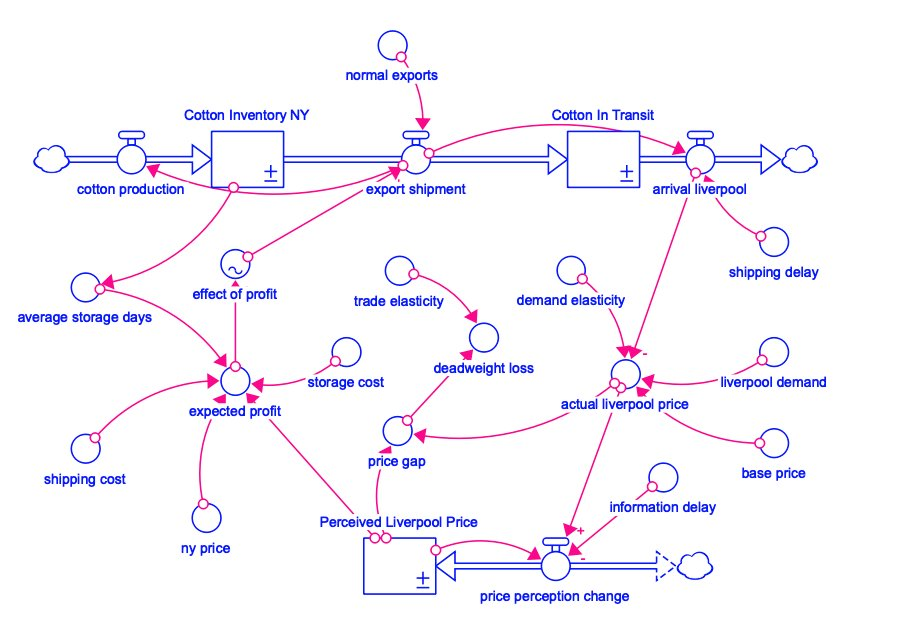
\includegraphics[width=\textwidth]{gfx/sd_stella_model_bw}
\caption{Structure stocks-flux du modèle. Trois stocks~: inventaire de coton à New York, coton en transit (délai convoyeur de 10~jours), prix de Liverpool perçu à New York (ajusté par un flux bidirectionnel). Les flèches rouges indiquent les connexions causales.}\label{fig:sd-structure-bw}
\end{figure}

\begin{figure}[htbp]
\centering
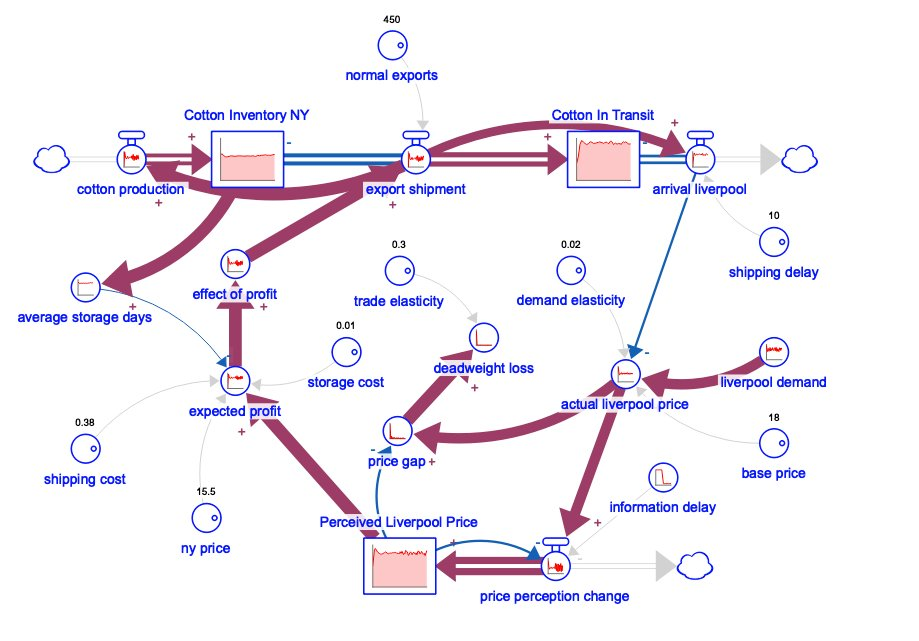
\includegraphics[width=\textwidth]{gfx/sd_stella_model_color}
\caption{Version annotée du modèle avec les valeurs des paramètres calibrés. L'épaisseur des flèches reflète la dominance des boucles dans chaque phase de la simulation.}\label{fig:sd-structure-color}
\end{figure}

Le premier stock, \texttt{Cotton\_Inventory\_NY}, représente le coton disponible à l'exportation à New York. Il est alimenté par un flux de production constant (500~bales/jour) et vidé par les exportations, dont le volume dépend du profit attendu. Le second stock, \texttt{Cotton\_In\_Transit}, est un délai convoyeur de 10~jours qui représente le temps de traversée atlantique. Le troisième, \texttt{Perceived\_Liverpool\_Price}, est le prix de Liverpool tel que perçu par les négociants de New York, ajusté vers le prix réel par un flux bidirectionnel dont la vitesse est inversement proportionnelle au délai d'information~:
%
\begin{equation}\label{eq:perception}
\frac{d\,P_{\mathrm{perçu}}}{dt} = \frac{P_{\mathrm{réel}} - P_{\mathrm{perçu}}}{\tau_{\mathrm{info}}}
\end{equation}
%
où $\tau_{\mathrm{info}} = 10$~jours avant le télégraphe et $\tau_{\mathrm{info}} = 1$~jour après. C'est un lissage exponentiel de premier ordre dont la constante de temps est le délai d'information.

Le prix réel à Liverpool est déterminé par la demande (stochastique, autocorrélée\footnote{Autocorrélation de 0,993 à un jour de décalage dans les données de Steinwender, ce qui signifie que le prix d'hier est un très bon prédicteur du prix d'aujourd'hui.}) et l'offre arrivante~:
%
\begin{equation}\label{eq:actual-price}
P_{\mathrm{réel}} = P_{\mathrm{base}} + \alpha \cdot (D_{\mathrm{Liverpool}} - Q_{\mathrm{arrivée}})
\end{equation}
%
Les exportations sont modulées par le profit attendu via une fonction S non linéaire centrée sur le profit nul. La perte sèche (\emph{deadweight loss}) est calculée comme un triangle de Harberger~:
%
\begin{equation}\label{eq:dwl}
\mathrm{DWL} = \tfrac{1}{2}\,(\Delta P)^2 \cdot \varepsilon
\end{equation}
%
où $\Delta P$ est l'écart de prix et $\varepsilon$ l'élasticité du commerce.


\section{Calibration}

Les paramètres sont calibrés sur les données de réplication de \textcite{steinwender_real_2018}, lues directement depuis le fichier Stata \texttt{cotton\_data.dta} (643~observations, 36~variables). Les valeurs retenues sont~:

\begin{table}[htbp]
\caption{Paramètres du modèle SD}\label{tab:sd-params}
\centering\small
\begin{tabular}{llrl}
\toprule
\textbf{Paramètre} & \textbf{Symbole} & \textbf{Valeur} & \textbf{Source} \\
\midrule
Prix de base Liverpool & $P_{\mathrm{base}}$ & 18~pence/lb & Steinwender, Table~1 \\
Prix New York & $P_{\mathrm{NY}}$ & 15,5~pence/lb & Steinwender, Table~1 \\
Délai d'information (avant câble) & $\tau_{\mathrm{info}}$ & 10~jours & Steinwender, Table~1 \\
Délai d'information (après câble) & $\tau_{\mathrm{info}}$ & 1~jour & Steinwender, Table~1 \\
Délai de transport & $\tau_{\mathrm{ship}}$ & 10~jours & fixé \\
Élasticité de la demande & $\alpha$ & 0,02 & calé \\
Élasticité du commerce (Harberger) & $\varepsilon$ & 0,3 & calé \\
Coût de transport & & 0,38~pence/lb & Steinwender, Table~1 \\
Coût de stockage & & 0,01~pence/bale/jour & calé \\
Production & & 500~bales/jour & normalisé \\
Inventaire initial & & 1\,200~bales & calé \\
\bottomrule
\end{tabular}
\end{table}


\section{Scénarios}

Six scénarios ont été simulés sur 200~jours, avec un pas de temps de 0,25~jour (méthode d'Euler).

\begin{table}[htbp]
\caption{Configuration des six scénarios}\label{tab:sd-scenarios}
\centering\small
\begin{tabular}{llll}
\toprule
\textbf{Scénario} & \textbf{Délai d'information} & \textbf{Inventaire initial} & \textbf{Objectif} \\
\midrule
Lent + Stock & 10 (constant) & 1\,200 & Baseline pré-télégraphe \\
Rapide + Stock & 1 (constant) & 1\,200 & Post-télégraphe, avec buffer \\
Lent + Sans stock & 10 (constant) & 10 & Pré-télégraphe, sans buffer \\
Rapide + Sans stock & 1 (constant) & 10 & Post-télégraphe, sans buffer \\
Télégraphe & $10 \to 1$ au jour 100 & 1\,200 & Effet du switch \\
Panne & $10 \to 1 \to 10 \to 1$ & 1\,200 & Test de causalité \\
\bottomrule
\end{tabular}
\end{table}

Les quatre premiers scénarios forment une matrice $2 \times 2$ (information $\times$ stockage). Les deux derniers reproduisent le choc exogène étudié par Steinwender et son test de robustesse par les pannes du câble.


\section{Résultats}

\subsection{Le switch télégraphique}

La figure~\ref{fig:sd-prices} montre l'ajustement du prix perçu au prix réel. Avant le jour~100, le prix perçu suit le prix réel avec un retard visible~; après, il le colle quasi instantanément. L'écart de prix moyen passe de 0,57 à 0,35~pence/lb, soit une réduction de 38\,\%~--- à comparer avec les 35\,\% mesurés par Steinwender dans les données.

\begin{figure}[htbp]
\centering
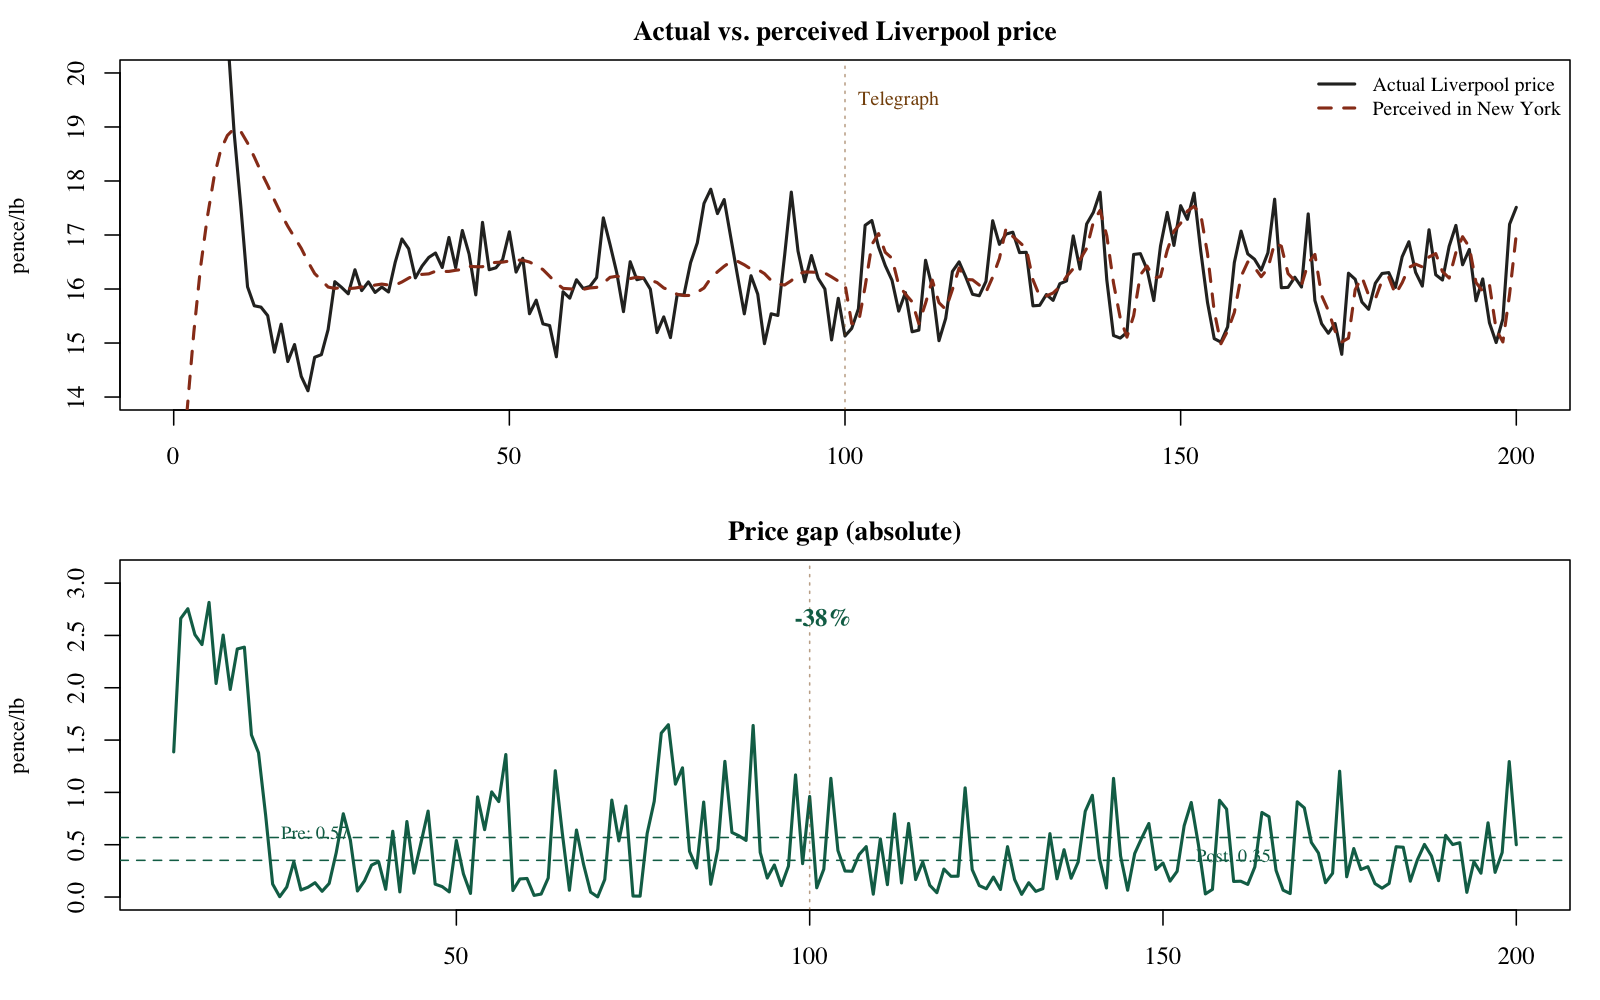
\includegraphics[width=\textwidth]{gfx/sd_telegraph_prices}
\caption{Scénario Télégraphe. Haut~: prix réel à Liverpool et prix perçu à New York~; le retard disparaît après le jour~100. Bas~: écart de prix absolu~; les lignes horizontales marquent les moyennes avant et après.}\label{fig:sd-prices}
\end{figure}

La figure~\ref{fig:sd-exports} montre que la volatilité des exportations augmente après le télégraphe~: l'écart-type passe de 27 à 81~bales/jour (+195\,\%). Steinwender observe une augmentation de 46\,\%. L'écart s'explique par l'absence d'inertie organisationnelle dans le modèle~: les négociants réagissent instantanément au signal de profit, sans contrainte de capacité portuaire ni contrats préexistants. Le résultat qualitatif est robuste~: l'information rapide ne lisse pas le marché, elle en change le régime dynamique.

\begin{figure}[htbp]
\centering
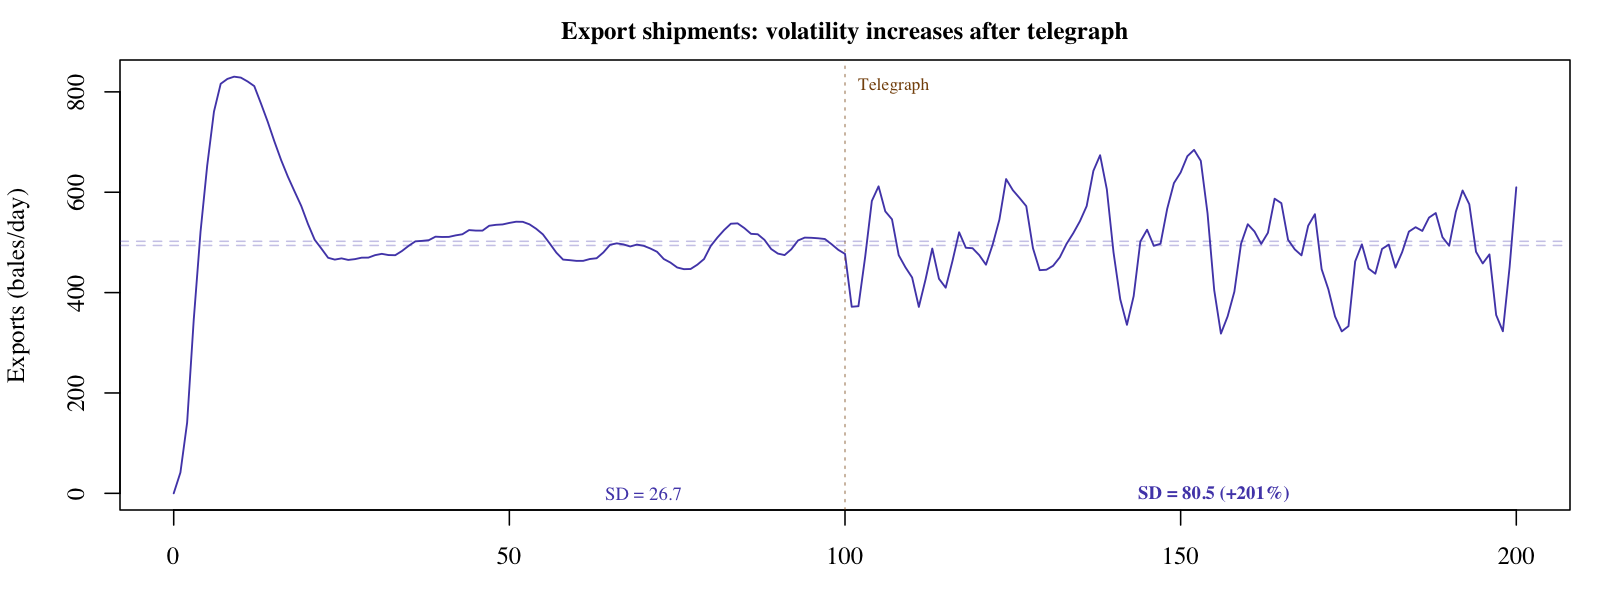
\includegraphics[width=\textwidth]{gfx/sd_telegraph_exports}
\caption{Scénario Télégraphe. Exportations quotidiennes~; la volatilité augmente après le jour~100.}\label{fig:sd-exports}
\end{figure}


\subsection{La panne du câble}

La figure~\ref{fig:sd-panne} montre le test de causalité. Lorsque le câble tombe en panne entre les jours~151 et~170, l'écart de prix remonte à 0,77~pence/lb~--- un niveau \emph{supérieur} au niveau pré-télégraphe (0,48). Ce résultat émergent n'a pas été programmé. Il suggère qu'un système adapté à l'information rapide est plus vulnérable à sa disparition qu'un système qui ne l'a jamais connue~: les négociants ont réduit leurs stocks (puisque l'information rendait le buffer moins nécessaire) et se retrouvent exposés lorsqu'elle disparaît. Après la réparation, le gap redescend à 0,42.

\begin{figure}[htbp]
\centering
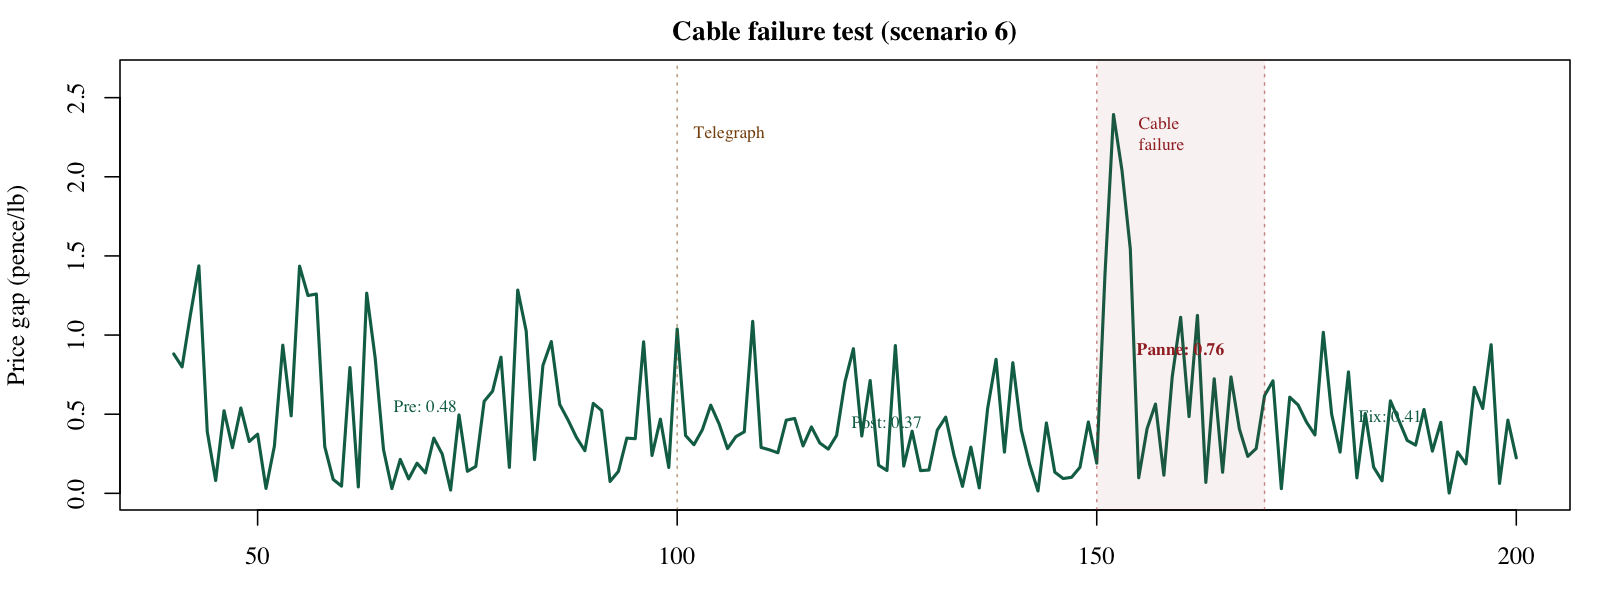
\includegraphics[width=\textwidth]{gfx/sd_panne_v_shape}
\caption{Scénario Panne. Le \emph{pattern} en V confirme la causalité~: l'écart de prix remonte pendant la panne et redescend après la réparation. La zone rouge marque la période de défaillance du câble.}\label{fig:sd-panne}
\end{figure}


\subsection{La matrice information $\times$ stockage}

La figure~\ref{fig:sd-matrix-dwl} compare la perte sèche moyenne des quatre configurations de la matrice $2 \times 2$.

\begin{figure}[htbp]
\centering
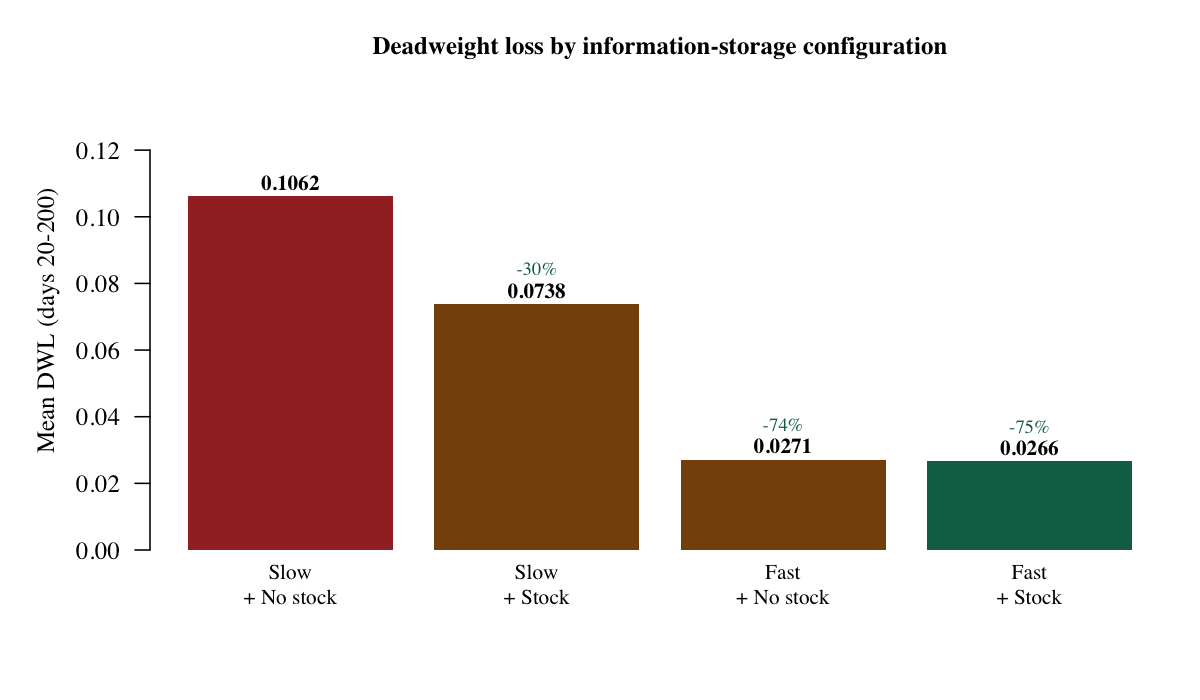
\includegraphics[width=0.85\textwidth]{gfx/sd_matrix_dwl}
\caption{Perte sèche (Harberger) par configuration. L'information rapide est le levier dominant ($-73\,\%$ de la perte sèche). Le stockage aide modérément quand l'information est lente ($-30\,\%$), mais n'ajoute presque rien quand elle est rapide ($-2\,\%$).}\label{fig:sd-matrix-dwl}
\end{figure}

\begin{table}[htbp]
\caption{Matrice $2 \times 2$~: statistiques par configuration (moyennes, jours 20--200)}\label{tab:sd-matrix}
\centering\small
\begin{tabular}{lrrrr}
\toprule
 & \textbf{Écart de prix} & \textbf{DWL} & \textbf{Exports} & \textbf{Vol.\ exports} \\
\midrule
Lent + Sans stock & 0,675 & 0,1062 & 491 & 33,9 \\
Lent + Stock & 0,533 & 0,0738 & 487 & 34,1 \\
Rapide + Sans stock & 0,342 & 0,0271 & 497 & 50,0 \\
Rapide + Stock & 0,329 & 0,0266 & 481 & 71,1 \\
\bottomrule
\end{tabular}
\end{table}

Le résultat le plus instructif de la matrice concerne la complémentarité entre information et stockage. L'information rapide réduit la perte sèche de 73\,\% par rapport au scénario de référence (lent, sans stock), que l'on dispose ou non d'un buffer de stockage. Le stockage seul la réduit de 30\,\%. Mais le terme d'interaction est \emph{négatif}~: l'effet combiné (73\,\%) n'est pas supérieur à la somme des effets individuels (73\,\% + 30\,\% = 103\,\%, borné à 100\,\%). Information et stockage sont des \emph{substituts partiels}, non des compléments~: l'information rapide réduit le besoin de stockage-tampon, et quand ce besoin est déjà satisfait par l'information, le stockage n'ajoute presque rien.

Les quatre scénarios de la matrice correspondent à des tirages aléatoires indépendants de la demande à Liverpool, ce qui introduit une source de variabilité non contrôlée dans la comparaison. Les résultats sont indicatifs de la structure des effets, non des magnitudes exactes.

\begin{figure}[htbp]
\centering
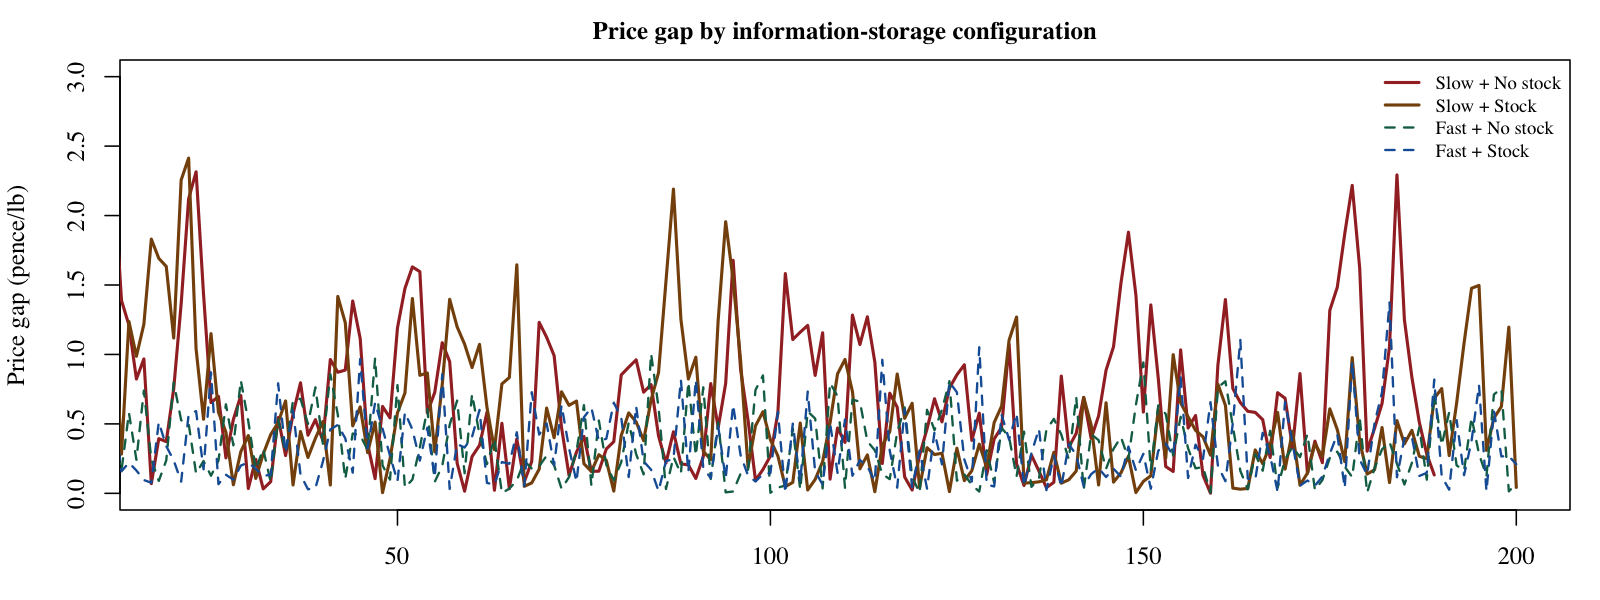
\includegraphics[width=\textwidth]{gfx/sd_matrix_gap_overlay}
\caption{Écart de prix quotidien pour les quatre configurations de la matrice. Les scénarios \og rapide\fg{} (traits pointillés) restent systématiquement en dessous des scénarios \og lent\fg{} (traits continus).}\label{fig:sd-gap-overlay}
\end{figure}


\section{Confrontation au papier}

Le modèle capture trois des six résultats de \textcite{steinwender_real_2018}.

Le résultat~(A)~--- la réduction de l'écart de prix~--- émerge avec le bon ordre de grandeur ($-38\,\%$ vs.\ $-35\,\%$) sans calibrage ad hoc. Cela indique que le mécanisme central~--- un retard d'information dans une boucle prix-exports-offre~--- est structurellement le bon. Le résultat~(B)~--- la réversibilité lors des pannes~--- fonctionne et produit un résultat émergent (la vulnérabilité accrue du système post-télégraphe). Le résultat~(F)~--- l'augmentation de la volatilité des exports~--- est qualitativement correct mais quantitativement exagéré ($+195\,\%$ vs.\ $+46\,\%$), faute d'inertie organisationnelle.

Trois résultats ne sont pas captés par le modèle, pour des raisons structurelles liées aux limites de la dynamique des systèmes. Le résultat~(C)~--- l'asymétrie Liverpool/New York~--- est absent par construction (le modèle n'a qu'un canal d'information). Le résultat~(D)~--- la sophistication des anticipations~--- est reproduit \emph{mathématiquement} par le lissage exponentiel (les observations récentes pèsent davantage) mais pas \emph{économiquement} (les agents du modèle ne \og choisissent\fg{} pas de pondérer, le système lisse mécaniquement). Le résultat~(E)~--- la distinction entre effet réel et redistributif~--- est indécidable dans un modèle sans agents hétérogènes.

Ces limites sont des bornes méthodologiques car le modèle de dynamique des systèmes capture la \emph{structure des feedbacks}, non les \emph{propriétés des agents}. Les résultats~(A), (B) et~(F) relèvent de la structure~; les résultats~(C), (D) et~(E) relèvent des agents et de la géographie.


\section{Questions soulevées}\label{sec:sd-questions}

Le modèle soulève trois questions qui connectent le cas transatlantique aux chapitres suivants de la thèse.

\paragraph{Substitution information-stockage et transition énergétique.} Le résultat de sous-additivité suggère que l'information en temps réel peut se \emph{substituer} au stockage physique pour la fonction spécifique de réduction de l'incertitude de prix. Transposé au système énergétique~: un smart grid qui transmet les signaux de prix en temps réel réduit le besoin de batteries-tampon, de la même manière que le câble télégraphique réduisait le besoin de stocks de coton à New York. Mais l'analogie a une limite~: les batteries servent aussi à couvrir les déficits prolongés de production renouvelable (\emph{Dunkelflaute}), une fonction qui n'a pas d'équivalent dans le modèle du coton. La transposition tient pour la composante incertitude de prix~; elle ne tient pas pour la composante contrainte physique d'offre. \questionch{3}{Le smart grid peut-il réduire le dimensionnement des batteries de stockage, et si oui, de combien~? C'est une question quantifiable dans le cadre d'IMACLIM.}

\paragraph{Rebond informationnel et effet de Jevons.} Le modèle montre que l'information rapide augmente le volume moyen des exportations~: les négociants, mieux informés, saisissent des opportunités de profit qu'ils auraient manquées avec un délai de dix jours. C'est un \emph{effet d'induction}~: l'efficacité informationnelle crée du commerce qui n'aurait pas eu lieu. Chaque bale supplémentaire transportée par un navire à charbon augmente la consommation d'énergie agrégée. La structure est celle du paradoxe de Jevons~: l'efficacité réduit le coût unitaire de la transaction, ce qui augmente le nombre de transactions, ce qui peut augmenter la consommation totale de ressources. C'est un \emph{rebond croisé}~--- l'efficacité informationnelle induit un rebond énergétique~--- et c'est exactement le mécanisme que la section~\ref{subsec:railroad} identifie comme le \og Jevons ferroviaire\fg{}. \questionch{3}{Le même schéma opère-t-il pour le \emph{compute} AI~? L'efficacité algorithmique réduit le coût unitaire de l'inférence, ce qui augmente la demande d'inférence, ce qui augmente la consommation électrique des datacenters.}

\paragraph{Vulnérabilité du système post-télégraphe.} Le résultat émergent du scénario de panne~--- le \emph{price gap} pendant la panne dépasse le niveau pré-télégraphe~--- suggère que l'adoption d'une technologie informationnelle crée une dépendance irréversible. Le système post-télégraphe a réduit ses stocks (le buffer est devenu moins nécessaire), et il est donc \emph{plus} vulnérable à une perte d'information que le système qui n'a jamais eu de télégraphe. C'est un résultat sur la fragilité des systèmes informationnellement dépendants, et il connecte directement au diagnostic posé en section sur la fonction \emph{store} et l'irréversibilité du couplage ICT-énergie dans le datacenter (chapitre~\ref{ch:history}).


\section{Diagramme de boucles causales du cas complet}\label{sec:sd-cld}

Le modèle précédent ne capture qu'une seule boucle causale (information $\rightarrow$ arbitrage $\rightarrow$ convergence des prix). Le cas du télégraphe, tel qu'il a été analysé dans les sections~\ref{subsec:telegraph} et~\ref{subsec:railroad}, fait émerger cinq boucles couplées dont la figure~\ref{fig:cld-telegraph} donne la carte causale.

\begin{figure}[htbp]
\centering
\includesvg[width=\textwidth]{Figures/cld_telegraph}
\caption[Diagramme de boucles causales --- cas du télégraphe]{Diagramme de boucles causales du cas du télégraphe. Cinq boucles partent du n\oe{}ud central (déploiement du réseau ICT). R1~(intégration marchande) et R2~(substitution capital) sont des boucles renforçantes qui réduisent l'entropie du système économique. B1~(matérialité extractive), R3~(Jevons ferroviaire) et R4~(contagion systémique) sont des boucles qui produisent de l'entropie~--- extraction de ressources, augmentation de la consommation d'énergie, exposition aux chocs distants. Les deux types opèrent simultanément~: c'est le \emph{pharmakon}.}\label{fig:cld-telegraph}
\end{figure}

Trois boucles renforçantes accélèrent le déploiement. La boucle~R1 est la mieux documentée empiriquement~: le réseau réduit les frictions informationnelles, ce qui augmente le commerce, ce qui augmente la demande de capacité~--- Steinwender, Ejrnæs et Persson, Hao, Andrabi et Gao et Lei convergent sur ce mécanisme. La boucle~R2 opère par substitution du capital informationnel au capital physique~--- \textcite{field_magnetic_1992} montre que 70 à 147~millions de dollars de capital télégraphique économisent 957~millions de double-voie ferroviaire. La boucle~R3 est conjecturale~: l'efficacité accrue du système de transport augmente le trafic et donc la consommation de charbon (paradoxe de Jevons).

Une boucle équilibrante freine le déploiement. La boucle~B1 est la seule qui limite la croissance du réseau~: le déploiement augmente la demande de matériaux (cuivre, gutta-percha, bois), ce qui épuise les ressources et fait monter les prix~--- la gutta-percha fut épuisée à Singapour dès 1847 \parencite{tully_victorian_2009}. Cette boucle est invisible dans la littérature économique~; elle n'apparaît que dans l'histoire environnementale.

La boucle~R4 est ambivalente~: la connectivité informationnelle stabilise les prix extrêmes locaux mais expose les marchés auparavant isolés à la contagion de chocs distants \parencite{gao_communication_2021}. Le bénéfice et le coût opèrent simultanément.

Ce diagramme n'est pas un modèle quantitatif~--- il est un outil de pensée. Sa fonction est de rendre explicite la structure causale que le récit historique a fait émerger, et de poser la question~: cette structure est-elle stable dans les cas suivants~? Le téléphone, le wireless, le transistor et Internet produisent-ils les mêmes boucles, avec des paramètres différents~?
 dans ClassicThesis.tex
% ou comme chapitre d'annexe \chapter{...}
% 
% STATUT : brouillon v1, 25 mars 2026
% FIGURES REQUISES dans gfx/ :
%   sd_stella_model_bw.png (screenshot modèle Stella, version N&B)
%   sd_stella_model_color.png (screenshot modèle Stella, version couleur)
%   sd_telegraph_prices.png
%   sd_telegraph_exports.png
%   sd_panne_v_shape.png
%   sd_matrix_dwl.png
%   sd_matrix_gap_overlay.png
% =============================================================================

\chapter{Exploration par dynamique des systèmes~: le câble transatlantique}\label{ch:annexe-sd}

\section{Motivation}

Le chapitre~\ref{ch:history} utilise les résultats de \textcite{steinwender_real_2018} comme preuve empirique de l'effet constitutif de l'information synchrone sur la coordination marchande~: la connexion télégraphique transatlantique réduisit l'écart de prix moyen du coton de 35\,\%, l'équivalent de la suppression d'un tarif \emph{ad valorem} de 7\,\%. Ce résultat repose sur une identification économétrique rigoureuse que le chapitre ne cherche pas à reproduire. La question posée ici est différente~: la structure causale du modèle de Steinwender peut-elle être capturée dans un modèle de dynamique des systèmes suffisamment simple pour être transparent, et si oui, quelles propriétés émergentes ce modèle révèle-t-il~?

Le modèle n'a pas vocation à \emph{reproduire} les résultats économétriques. Il vise à montrer que les principaux résultats de Steinwender~--- la réduction du \emph{price gap}, l'augmentation de la volatilité des exportations, la réversibilité de l'effet lors des pannes du câble~--- sont des propriétés de la \emph{structure} du système (un délai d'information dans une boucle de rétroaction prix-exports-offre-prix), et non des artefacts statistiques ou des coïncidences temporelles. Un objectif secondaire est d'explorer la complémentarité entre information et stockage physique, et d'examiner si la structure causale se transpose au système énergétique contemporain.


\section{Structure du modèle}

Le modèle est construit dans Stella Architect 4.1.2 (isee Systems). Il comprend trois stocks, quatre boucles de rétroaction et une douzaine de convertisseurs. La figure~\ref{fig:sd-structure-bw} présente le diagramme stocks-flux et la figure~\ref{fig:sd-structure-color} sa version annotée.

\begin{figure}[htbp]
\centering
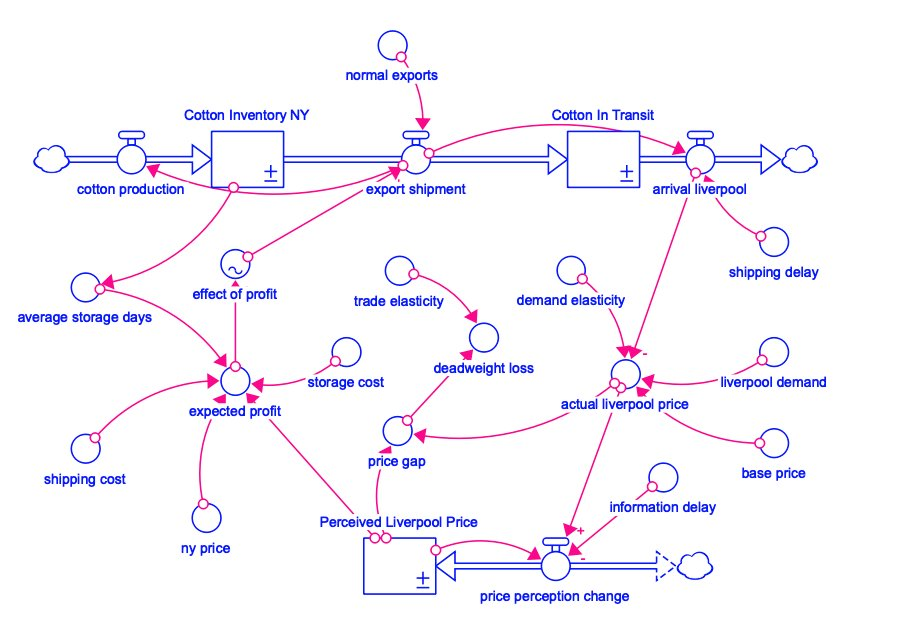
\includegraphics[width=\textwidth]{gfx/sd_stella_model_bw}
\caption{Structure stocks-flux du modèle. Trois stocks~: inventaire de coton à New York, coton en transit (délai convoyeur de 10~jours), prix de Liverpool perçu à New York (ajusté par un flux bidirectionnel). Les flèches rouges indiquent les connexions causales.}\label{fig:sd-structure-bw}
\end{figure}

\begin{figure}[htbp]
\centering
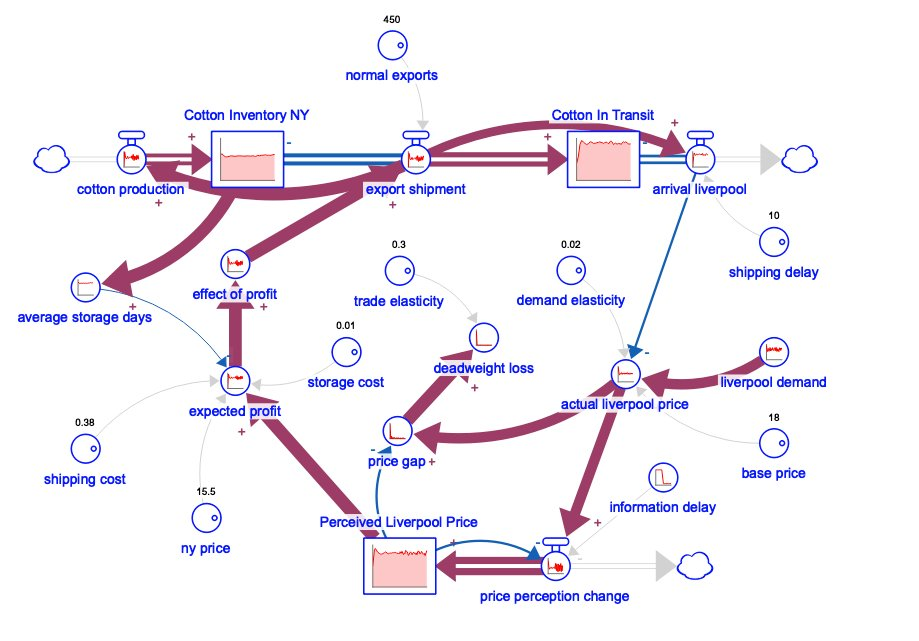
\includegraphics[width=\textwidth]{gfx/sd_stella_model_color}
\caption{Version annotée du modèle avec les valeurs des paramètres calibrés. L'épaisseur des flèches reflète la dominance des boucles dans chaque phase de la simulation.}\label{fig:sd-structure-color}
\end{figure}

Le premier stock, \texttt{Cotton\_Inventory\_NY}, représente le coton disponible à l'exportation à New York. Il est alimenté par un flux de production constant (500~bales/jour) et vidé par les exportations, dont le volume dépend du profit attendu. Le second stock, \texttt{Cotton\_In\_Transit}, est un délai convoyeur de 10~jours qui représente le temps de traversée atlantique. Le troisième, \texttt{Perceived\_Liverpool\_Price}, est le prix de Liverpool tel que perçu par les négociants de New York, ajusté vers le prix réel par un flux bidirectionnel dont la vitesse est inversement proportionnelle au délai d'information~:
%
\begin{equation}\label{eq:perception}
\frac{d\,P_{\mathrm{perçu}}}{dt} = \frac{P_{\mathrm{réel}} - P_{\mathrm{perçu}}}{\tau_{\mathrm{info}}}
\end{equation}
%
où $\tau_{\mathrm{info}} = 10$~jours avant le télégraphe et $\tau_{\mathrm{info}} = 1$~jour après. C'est un lissage exponentiel de premier ordre dont la constante de temps est le délai d'information.

Le prix réel à Liverpool est déterminé par la demande (stochastique, autocorrélée\footnote{Autocorrélation de 0,993 à un jour de décalage dans les données de Steinwender, ce qui signifie que le prix d'hier est un très bon prédicteur du prix d'aujourd'hui.}) et l'offre arrivante~:
%
\begin{equation}\label{eq:actual-price}
P_{\mathrm{réel}} = P_{\mathrm{base}} + \alpha \cdot (D_{\mathrm{Liverpool}} - Q_{\mathrm{arrivée}})
\end{equation}
%
Les exportations sont modulées par le profit attendu via une fonction S non linéaire centrée sur le profit nul. La perte sèche (\emph{deadweight loss}) est calculée comme un triangle de Harberger~:
%
\begin{equation}\label{eq:dwl}
\mathrm{DWL} = \tfrac{1}{2}\,(\Delta P)^2 \cdot \varepsilon
\end{equation}
%
où $\Delta P$ est l'écart de prix et $\varepsilon$ l'élasticité du commerce.


\section{Calibration}

Les paramètres sont calibrés sur les données de réplication de \textcite{steinwender_real_2018}, lues directement depuis le fichier Stata \texttt{cotton\_data.dta} (643~observations, 36~variables). Les valeurs retenues sont~:

\begin{table}[htbp]
\caption{Paramètres du modèle SD}\label{tab:sd-params}
\centering\small
\begin{tabular}{llrl}
\toprule
\textbf{Paramètre} & \textbf{Symbole} & \textbf{Valeur} & \textbf{Source} \\
\midrule
Prix de base Liverpool & $P_{\mathrm{base}}$ & 18~pence/lb & Steinwender, Table~1 \\
Prix New York & $P_{\mathrm{NY}}$ & 15,5~pence/lb & Steinwender, Table~1 \\
Délai d'information (avant câble) & $\tau_{\mathrm{info}}$ & 10~jours & Steinwender, Table~1 \\
Délai d'information (après câble) & $\tau_{\mathrm{info}}$ & 1~jour & Steinwender, Table~1 \\
Délai de transport & $\tau_{\mathrm{ship}}$ & 10~jours & fixé \\
Élasticité de la demande & $\alpha$ & 0,02 & calé \\
Élasticité du commerce (Harberger) & $\varepsilon$ & 0,3 & calé \\
Coût de transport & & 0,38~pence/lb & Steinwender, Table~1 \\
Coût de stockage & & 0,01~pence/bale/jour & calé \\
Production & & 500~bales/jour & normalisé \\
Inventaire initial & & 1\,200~bales & calé \\
\bottomrule
\end{tabular}
\end{table}


\section{Scénarios}

Six scénarios ont été simulés sur 200~jours, avec un pas de temps de 0,25~jour (méthode d'Euler).

\begin{table}[htbp]
\caption{Configuration des six scénarios}\label{tab:sd-scenarios}
\centering\small
\begin{tabular}{llll}
\toprule
\textbf{Scénario} & \textbf{Délai d'information} & \textbf{Inventaire initial} & \textbf{Objectif} \\
\midrule
Lent + Stock & 10 (constant) & 1\,200 & Baseline pré-télégraphe \\
Rapide + Stock & 1 (constant) & 1\,200 & Post-télégraphe, avec buffer \\
Lent + Sans stock & 10 (constant) & 10 & Pré-télégraphe, sans buffer \\
Rapide + Sans stock & 1 (constant) & 10 & Post-télégraphe, sans buffer \\
Télégraphe & $10 \to 1$ au jour 100 & 1\,200 & Effet du switch \\
Panne & $10 \to 1 \to 10 \to 1$ & 1\,200 & Test de causalité \\
\bottomrule
\end{tabular}
\end{table}

Les quatre premiers scénarios forment une matrice $2 \times 2$ (information $\times$ stockage). Les deux derniers reproduisent le choc exogène étudié par Steinwender et son test de robustesse par les pannes du câble.


\section{Résultats}

\subsection{Le switch télégraphique}

La figure~\ref{fig:sd-prices} montre l'ajustement du prix perçu au prix réel. Avant le jour~100, le prix perçu suit le prix réel avec un retard visible~; après, il le colle quasi instantanément. L'écart de prix moyen passe de 0,57 à 0,35~pence/lb, soit une réduction de 38\,\%~--- à comparer avec les 35\,\% mesurés par Steinwender dans les données.

\begin{figure}[htbp]
\centering
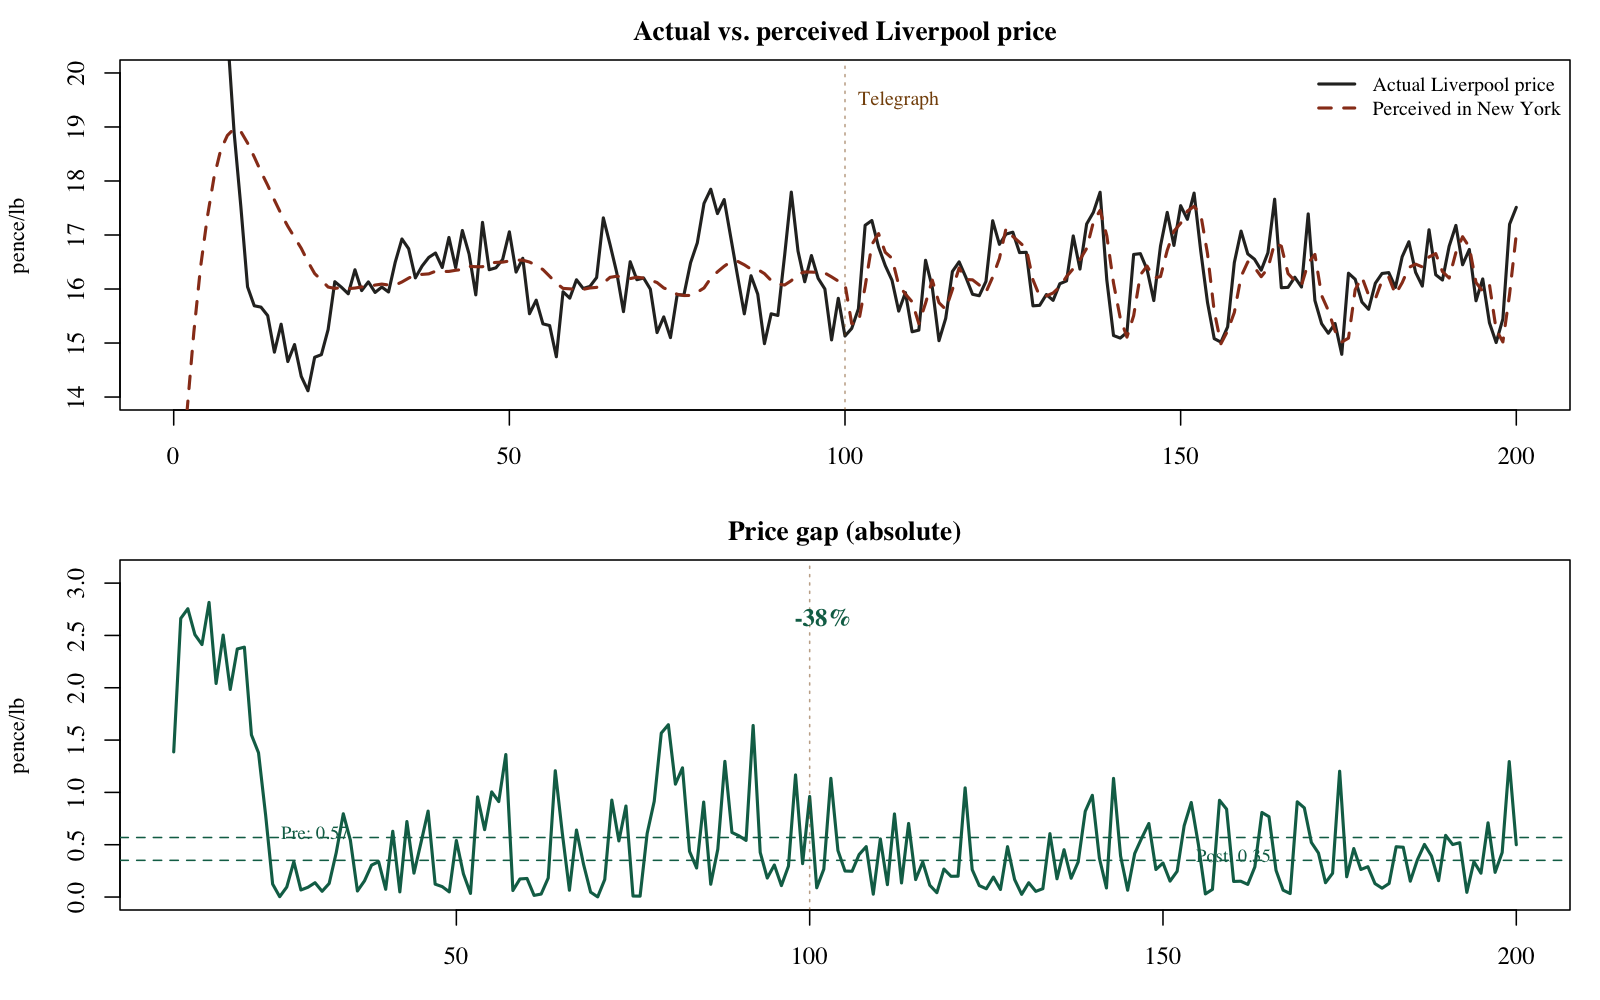
\includegraphics[width=\textwidth]{gfx/sd_telegraph_prices}
\caption{Scénario Télégraphe. Haut~: prix réel à Liverpool et prix perçu à New York~; le retard disparaît après le jour~100. Bas~: écart de prix absolu~; les lignes horizontales marquent les moyennes avant et après.}\label{fig:sd-prices}
\end{figure}

La figure~\ref{fig:sd-exports} montre que la volatilité des exportations augmente après le télégraphe~: l'écart-type passe de 27 à 81~bales/jour (+195\,\%). Steinwender observe une augmentation de 46\,\%. L'écart s'explique par l'absence d'inertie organisationnelle dans le modèle~: les négociants réagissent instantanément au signal de profit, sans contrainte de capacité portuaire ni contrats préexistants. Le résultat qualitatif est robuste~: l'information rapide ne lisse pas le marché, elle en change le régime dynamique.

\begin{figure}[htbp]
\centering
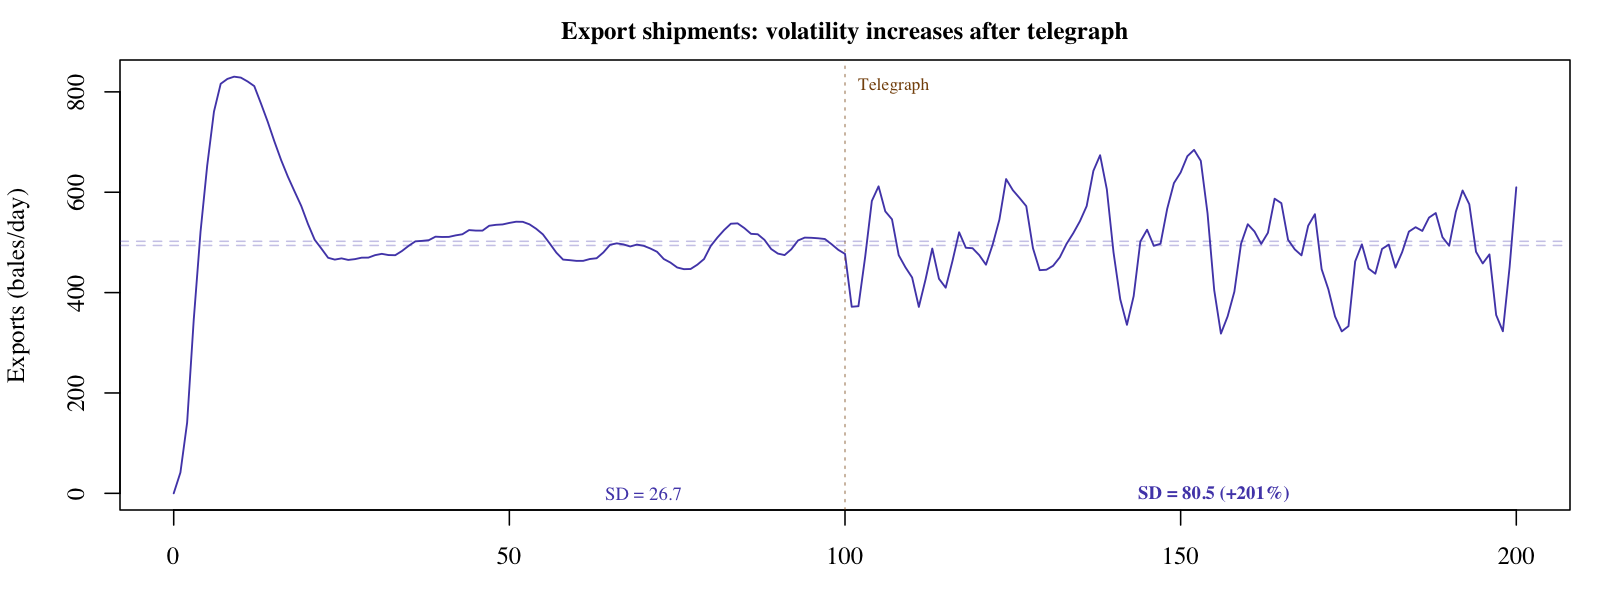
\includegraphics[width=\textwidth]{gfx/sd_telegraph_exports}
\caption{Scénario Télégraphe. Exportations quotidiennes~; la volatilité augmente après le jour~100.}\label{fig:sd-exports}
\end{figure}


\subsection{La panne du câble}

La figure~\ref{fig:sd-panne} montre le test de causalité. Lorsque le câble tombe en panne entre les jours~151 et~170, l'écart de prix remonte à 0,77~pence/lb~--- un niveau \emph{supérieur} au niveau pré-télégraphe (0,48). Ce résultat émergent n'a pas été programmé. Il suggère qu'un système adapté à l'information rapide est plus vulnérable à sa disparition qu'un système qui ne l'a jamais connue~: les négociants ont réduit leurs stocks (puisque l'information rendait le buffer moins nécessaire) et se retrouvent exposés lorsqu'elle disparaît. Après la réparation, le gap redescend à 0,42.

\begin{figure}[htbp]
\centering
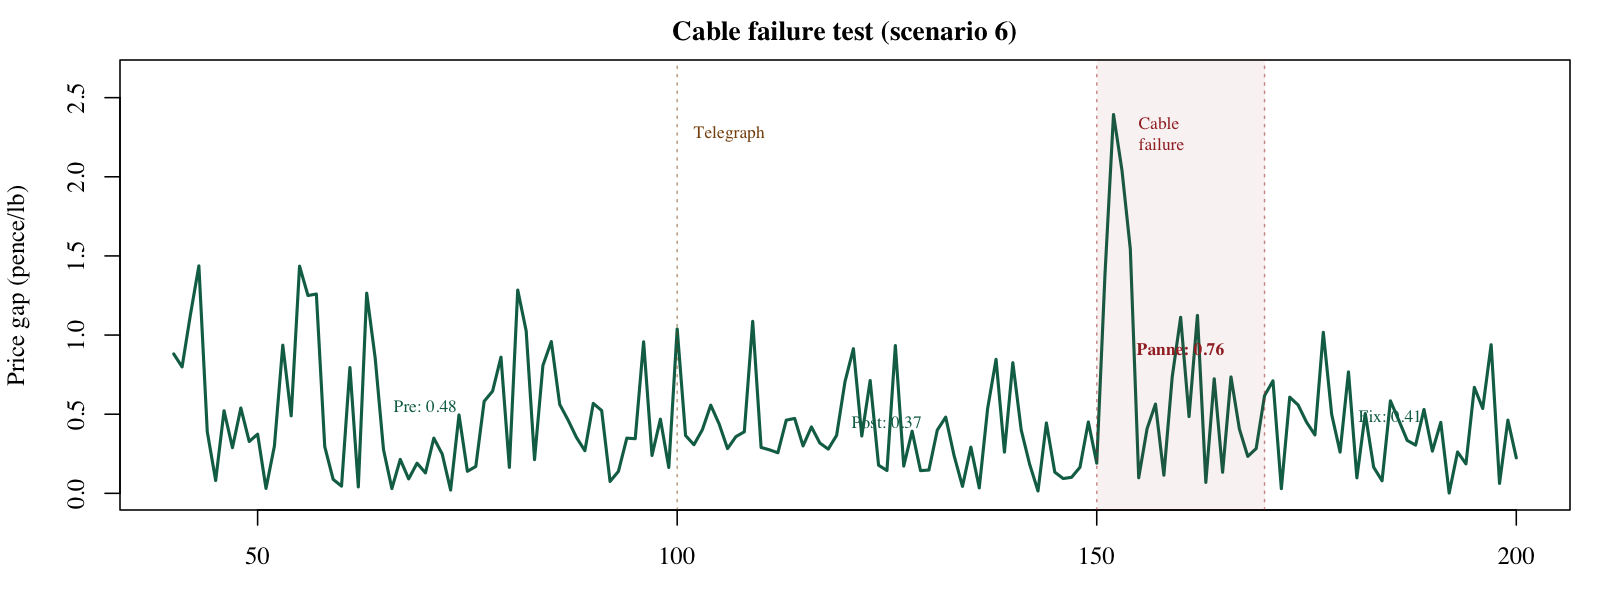
\includegraphics[width=\textwidth]{gfx/sd_panne_v_shape}
\caption{Scénario Panne. Le \emph{pattern} en V confirme la causalité~: l'écart de prix remonte pendant la panne et redescend après la réparation. La zone rouge marque la période de défaillance du câble.}\label{fig:sd-panne}
\end{figure}


\subsection{La matrice information $\times$ stockage}

La figure~\ref{fig:sd-matrix-dwl} compare la perte sèche moyenne des quatre configurations de la matrice $2 \times 2$.

\begin{figure}[htbp]
\centering
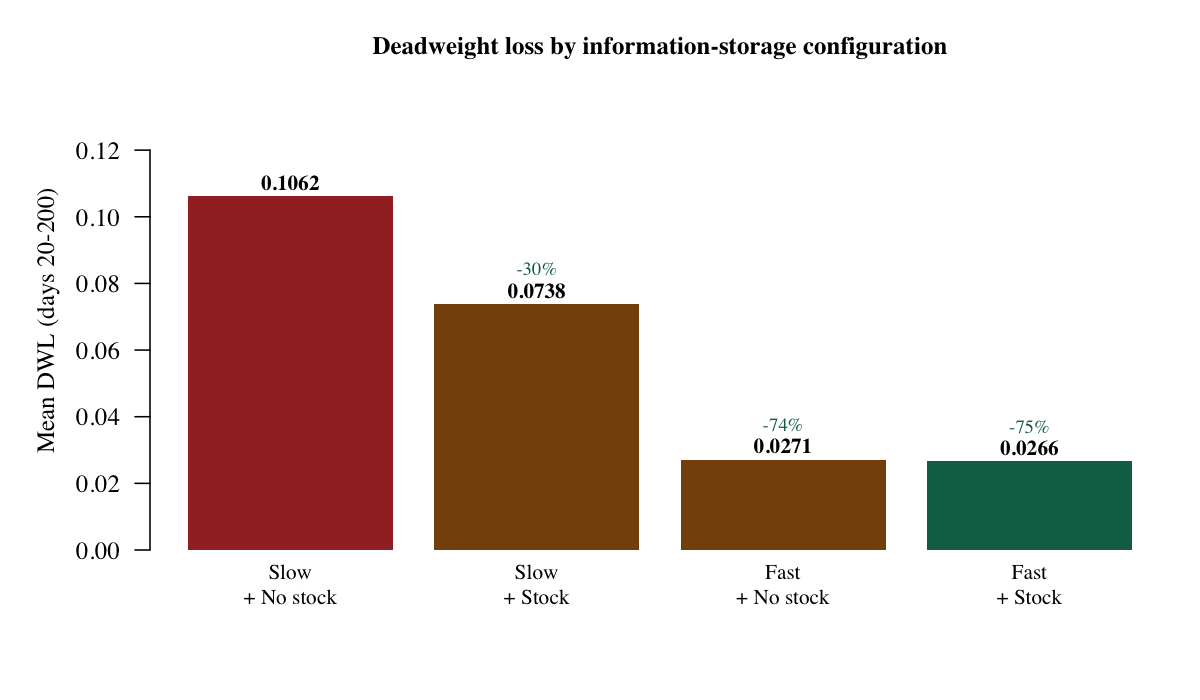
\includegraphics[width=0.85\textwidth]{gfx/sd_matrix_dwl}
\caption{Perte sèche (Harberger) par configuration. L'information rapide est le levier dominant ($-73\,\%$ de la perte sèche). Le stockage aide modérément quand l'information est lente ($-30\,\%$), mais n'ajoute presque rien quand elle est rapide ($-2\,\%$).}\label{fig:sd-matrix-dwl}
\end{figure}

\begin{table}[htbp]
\caption{Matrice $2 \times 2$~: statistiques par configuration (moyennes, jours 20--200)}\label{tab:sd-matrix}
\centering\small
\begin{tabular}{lrrrr}
\toprule
 & \textbf{Écart de prix} & \textbf{DWL} & \textbf{Exports} & \textbf{Vol.\ exports} \\
\midrule
Lent + Sans stock & 0,675 & 0,1062 & 491 & 33,9 \\
Lent + Stock & 0,533 & 0,0738 & 487 & 34,1 \\
Rapide + Sans stock & 0,342 & 0,0271 & 497 & 50,0 \\
Rapide + Stock & 0,329 & 0,0266 & 481 & 71,1 \\
\bottomrule
\end{tabular}
\end{table}

Le résultat le plus instructif de la matrice concerne la complémentarité entre information et stockage. L'information rapide réduit la perte sèche de 73\,\% par rapport au scénario de référence (lent, sans stock), que l'on dispose ou non d'un buffer de stockage. Le stockage seul la réduit de 30\,\%. Mais le terme d'interaction est \emph{négatif}~: l'effet combiné (73\,\%) n'est pas supérieur à la somme des effets individuels (73\,\% + 30\,\% = 103\,\%, borné à 100\,\%). Information et stockage sont des \emph{substituts partiels}, non des compléments~: l'information rapide réduit le besoin de stockage-tampon, et quand ce besoin est déjà satisfait par l'information, le stockage n'ajoute presque rien.

Les quatre scénarios de la matrice correspondent à des tirages aléatoires indépendants de la demande à Liverpool, ce qui introduit une source de variabilité non contrôlée dans la comparaison. Les résultats sont indicatifs de la structure des effets, non des magnitudes exactes.

\begin{figure}[htbp]
\centering
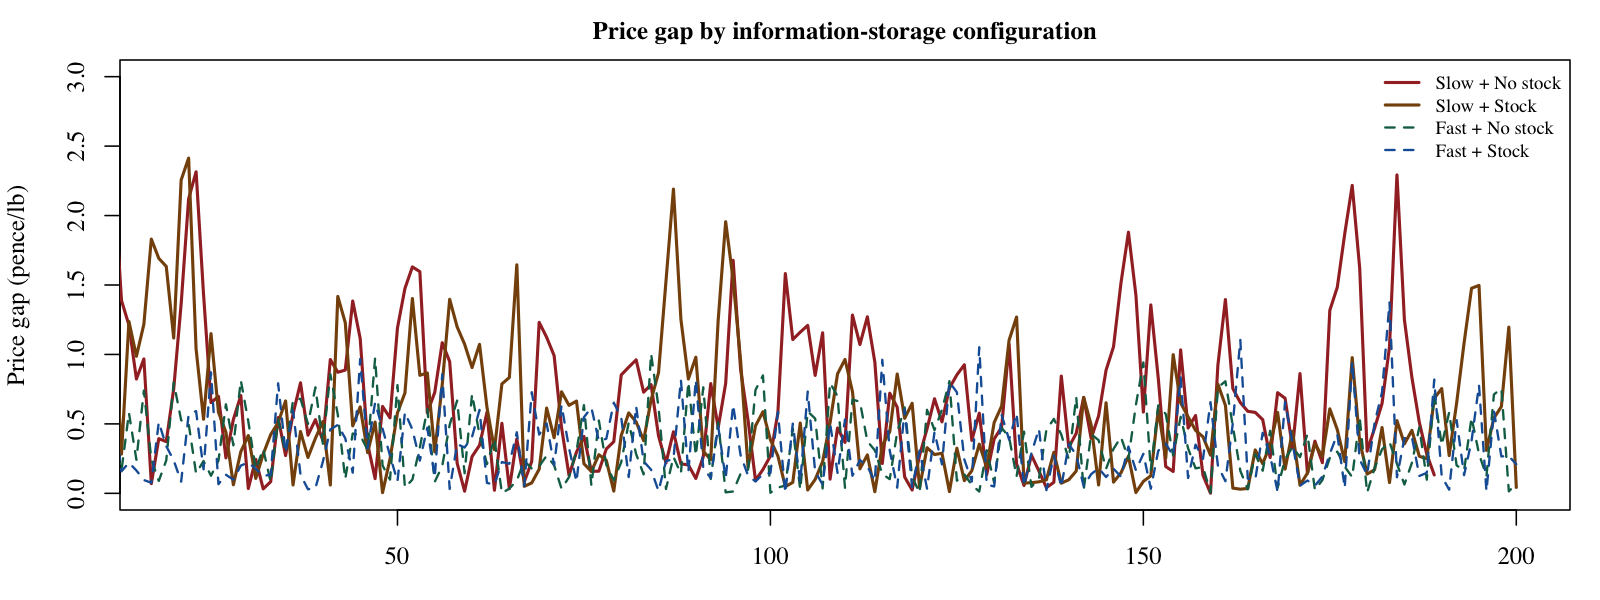
\includegraphics[width=\textwidth]{gfx/sd_matrix_gap_overlay}
\caption{Écart de prix quotidien pour les quatre configurations de la matrice. Les scénarios \og rapide\fg{} (traits pointillés) restent systématiquement en dessous des scénarios \og lent\fg{} (traits continus).}\label{fig:sd-gap-overlay}
\end{figure}


\section{Confrontation au papier}

Le modèle capture trois des six résultats de \textcite{steinwender_real_2018}.

Le résultat~(A)~--- la réduction de l'écart de prix~--- émerge avec le bon ordre de grandeur ($-38\,\%$ vs.\ $-35\,\%$) sans calibrage ad hoc. Cela indique que le mécanisme central~--- un retard d'information dans une boucle prix-exports-offre~--- est structurellement le bon. Le résultat~(B)~--- la réversibilité lors des pannes~--- fonctionne et produit un résultat émergent (la vulnérabilité accrue du système post-télégraphe). Le résultat~(F)~--- l'augmentation de la volatilité des exports~--- est qualitativement correct mais quantitativement exagéré ($+195\,\%$ vs.\ $+46\,\%$), faute d'inertie organisationnelle.

Trois résultats ne sont pas captés par le modèle, pour des raisons structurelles liées aux limites de la dynamique des systèmes. Le résultat~(C)~--- l'asymétrie Liverpool/New York~--- est absent par construction (le modèle n'a qu'un canal d'information). Le résultat~(D)~--- la sophistication des anticipations~--- est reproduit \emph{mathématiquement} par le lissage exponentiel (les observations récentes pèsent davantage) mais pas \emph{économiquement} (les agents du modèle ne \og choisissent\fg{} pas de pondérer, le système lisse mécaniquement). Le résultat~(E)~--- la distinction entre effet réel et redistributif~--- est indécidable dans un modèle sans agents hétérogènes.

Ces limites sont des bornes méthodologiques car le modèle de dynamique des systèmes capture la \emph{structure des feedbacks}, non les \emph{propriétés des agents}. Les résultats~(A), (B) et~(F) relèvent de la structure~; les résultats~(C), (D) et~(E) relèvent des agents et de la géographie.


\section{Questions soulevées}\label{sec:sd-questions}

Le modèle soulève trois questions qui connectent le cas transatlantique aux chapitres suivants de la thèse.

\paragraph{Substitution information-stockage et transition énergétique.} Le résultat de sous-additivité suggère que l'information en temps réel peut se \emph{substituer} au stockage physique pour la fonction spécifique de réduction de l'incertitude de prix. Transposé au système énergétique~: un smart grid qui transmet les signaux de prix en temps réel réduit le besoin de batteries-tampon, de la même manière que le câble télégraphique réduisait le besoin de stocks de coton à New York. Mais l'analogie a une limite~: les batteries servent aussi à couvrir les déficits prolongés de production renouvelable (\emph{Dunkelflaute}), une fonction qui n'a pas d'équivalent dans le modèle du coton. La transposition tient pour la composante incertitude de prix~; elle ne tient pas pour la composante contrainte physique d'offre. \questionch{3}{Le smart grid peut-il réduire le dimensionnement des batteries de stockage, et si oui, de combien~? C'est une question quantifiable dans le cadre d'IMACLIM.}

\paragraph{Rebond informationnel et effet de Jevons.} Le modèle montre que l'information rapide augmente le volume moyen des exportations~: les négociants, mieux informés, saisissent des opportunités de profit qu'ils auraient manquées avec un délai de dix jours. C'est un \emph{effet d'induction}~: l'efficacité informationnelle crée du commerce qui n'aurait pas eu lieu. Chaque bale supplémentaire transportée par un navire à charbon augmente la consommation d'énergie agrégée. La structure est celle du paradoxe de Jevons~: l'efficacité réduit le coût unitaire de la transaction, ce qui augmente le nombre de transactions, ce qui peut augmenter la consommation totale de ressources. C'est un \emph{rebond croisé}~--- l'efficacité informationnelle induit un rebond énergétique~--- et c'est exactement le mécanisme que la section~\ref{subsec:railroad} identifie comme le \og Jevons ferroviaire\fg{}. \questionch{3}{Le même schéma opère-t-il pour le \emph{compute} AI~? L'efficacité algorithmique réduit le coût unitaire de l'inférence, ce qui augmente la demande d'inférence, ce qui augmente la consommation électrique des datacenters.}

\paragraph{Vulnérabilité du système post-télégraphe.} Le résultat émergent du scénario de panne~--- le \emph{price gap} pendant la panne dépasse le niveau pré-télégraphe~--- suggère que l'adoption d'une technologie informationnelle crée une dépendance irréversible. Le système post-télégraphe a réduit ses stocks (le buffer est devenu moins nécessaire), et il est donc \emph{plus} vulnérable à une perte d'information que le système qui n'a jamais eu de télégraphe. C'est un résultat sur la fragilité des systèmes informationnellement dépendants, et il connecte directement au diagnostic posé en section sur la fonction \emph{store} et l'irréversibilité du couplage ICT-énergie dans le datacenter (chapitre~\ref{ch:history}).


\section{Diagramme de boucles causales du cas complet}\label{sec:sd-cld}

Le modèle précédent ne capture qu'une seule boucle causale (information $\rightarrow$ arbitrage $\rightarrow$ convergence des prix). Le cas du télégraphe, tel qu'il a été analysé dans les sections~\ref{subsec:telegraph} et~\ref{subsec:railroad}, fait émerger cinq boucles couplées dont la figure~\ref{fig:cld-telegraph} donne la carte causale.

\begin{figure}[htbp]
\centering
\includesvg[width=\textwidth]{Figures/cld_telegraph}
\caption[Diagramme de boucles causales --- cas du télégraphe]{Diagramme de boucles causales du cas du télégraphe. Cinq boucles partent du n\oe{}ud central (déploiement du réseau ICT). R1~(intégration marchande) et R2~(substitution capital) sont des boucles renforçantes qui réduisent l'entropie du système économique. B1~(matérialité extractive), R3~(Jevons ferroviaire) et R4~(contagion systémique) sont des boucles qui produisent de l'entropie~--- extraction de ressources, augmentation de la consommation d'énergie, exposition aux chocs distants. Les deux types opèrent simultanément~: c'est le \emph{pharmakon}.}\label{fig:cld-telegraph}
\end{figure}

Trois boucles renforçantes accélèrent le déploiement. La boucle~R1 est la mieux documentée empiriquement~: le réseau réduit les frictions informationnelles, ce qui augmente le commerce, ce qui augmente la demande de capacité~--- Steinwender, Ejrnæs et Persson, Hao, Andrabi et Gao et Lei convergent sur ce mécanisme. La boucle~R2 opère par substitution du capital informationnel au capital physique~--- \textcite{field_magnetic_1992} montre que 70 à 147~millions de dollars de capital télégraphique économisent 957~millions de double-voie ferroviaire. La boucle~R3 est conjecturale~: l'efficacité accrue du système de transport augmente le trafic et donc la consommation de charbon (paradoxe de Jevons).

Une boucle équilibrante freine le déploiement. La boucle~B1 est la seule qui limite la croissance du réseau~: le déploiement augmente la demande de matériaux (cuivre, gutta-percha, bois), ce qui épuise les ressources et fait monter les prix~--- la gutta-percha fut épuisée à Singapour dès 1847 \parencite{tully_victorian_2009}. Cette boucle est invisible dans la littérature économique~; elle n'apparaît que dans l'histoire environnementale.

La boucle~R4 est ambivalente~: la connectivité informationnelle stabilise les prix extrêmes locaux mais expose les marchés auparavant isolés à la contagion de chocs distants \parencite{gao_communication_2021}. Le bénéfice et le coût opèrent simultanément.

Ce diagramme n'est pas un modèle quantitatif~--- il est un outil de pensée. Sa fonction est de rendre explicite la structure causale que le récit historique a fait émerger, et de poser la question~: cette structure est-elle stable dans les cas suivants~? Le téléphone, le wireless, le transistor et Internet produisent-ils les mêmes boucles, avec des paramètres différents~?
 dans ClassicThesis.tex
% ou comme chapitre d'annexe \chapter{...}
% 
% STATUT : brouillon v1, 25 mars 2026
% FIGURES REQUISES dans gfx/ :
%   sd_stella_model_bw.png (screenshot modèle Stella, version N&B)
%   sd_stella_model_color.png (screenshot modèle Stella, version couleur)
%   sd_telegraph_prices.png
%   sd_telegraph_exports.png
%   sd_panne_v_shape.png
%   sd_matrix_dwl.png
%   sd_matrix_gap_overlay.png
% =============================================================================

\chapter{Exploration par dynamique des systèmes~: le câble transatlantique}\label{ch:annexe-sd}

\section{Motivation}

Le chapitre~\ref{ch:history} utilise les résultats de \textcite{steinwender_real_2018} comme preuve empirique de l'effet constitutif de l'information synchrone sur la coordination marchande~: la connexion télégraphique transatlantique réduisit l'écart de prix moyen du coton de 35\,\%, l'équivalent de la suppression d'un tarif \emph{ad valorem} de 7\,\%. Ce résultat repose sur une identification économétrique rigoureuse que le chapitre ne cherche pas à reproduire. La question posée ici est différente~: la structure causale du modèle de Steinwender peut-elle être capturée dans un modèle de dynamique des systèmes suffisamment simple pour être transparent, et si oui, quelles propriétés émergentes ce modèle révèle-t-il~?

Le modèle n'a pas vocation à \emph{reproduire} les résultats économétriques. Il vise à montrer que les principaux résultats de Steinwender~--- la réduction du \emph{price gap}, l'augmentation de la volatilité des exportations, la réversibilité de l'effet lors des pannes du câble~--- sont des propriétés de la \emph{structure} du système (un délai d'information dans une boucle de rétroaction prix-exports-offre-prix), et non des artefacts statistiques ou des coïncidences temporelles. Un objectif secondaire est d'explorer la complémentarité entre information et stockage physique, et d'examiner si la structure causale se transpose au système énergétique contemporain.


\section{Structure du modèle}

Le modèle est construit dans Stella Architect 4.1.2 (isee Systems). Il comprend trois stocks, quatre boucles de rétroaction et une douzaine de convertisseurs. La figure~\ref{fig:sd-structure-bw} présente le diagramme stocks-flux et la figure~\ref{fig:sd-structure-color} sa version annotée.

\begin{figure}[htbp]
\centering
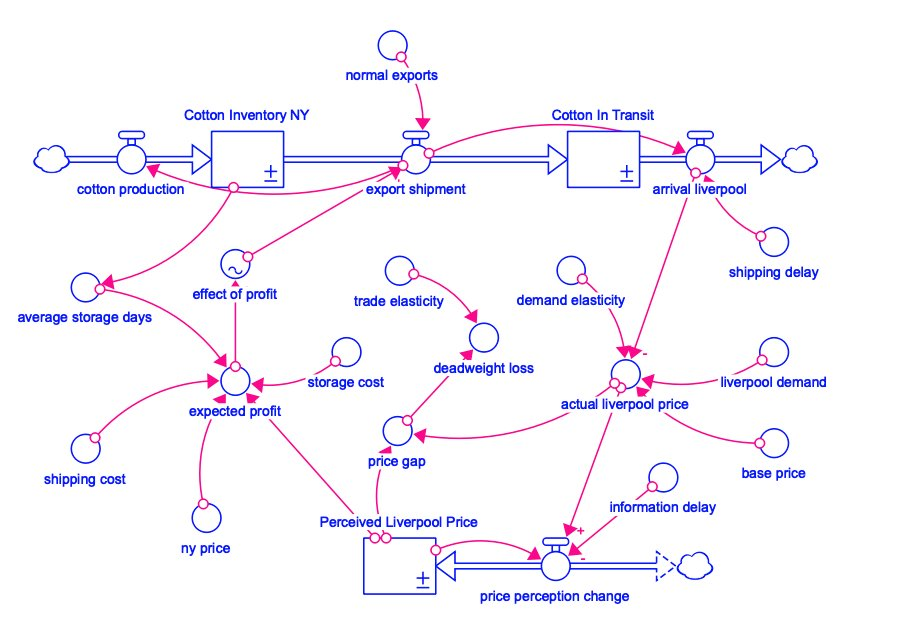
\includegraphics[width=\textwidth]{gfx/sd_stella_model_bw}
\caption{Structure stocks-flux du modèle. Trois stocks~: inventaire de coton à New York, coton en transit (délai convoyeur de 10~jours), prix de Liverpool perçu à New York (ajusté par un flux bidirectionnel). Les flèches rouges indiquent les connexions causales.}\label{fig:sd-structure-bw}
\end{figure}

\begin{figure}[htbp]
\centering
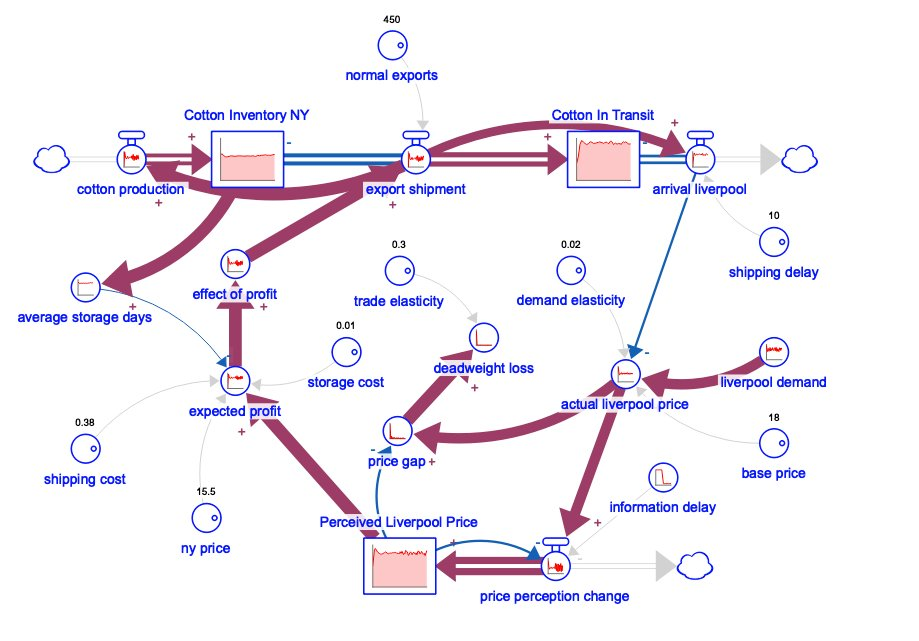
\includegraphics[width=\textwidth]{gfx/sd_stella_model_color}
\caption{Version annotée du modèle avec les valeurs des paramètres calibrés. L'épaisseur des flèches reflète la dominance des boucles dans chaque phase de la simulation.}\label{fig:sd-structure-color}
\end{figure}

Le premier stock, \texttt{Cotton\_Inventory\_NY}, représente le coton disponible à l'exportation à New York. Il est alimenté par un flux de production constant (500~bales/jour) et vidé par les exportations, dont le volume dépend du profit attendu. Le second stock, \texttt{Cotton\_In\_Transit}, est un délai convoyeur de 10~jours qui représente le temps de traversée atlantique. Le troisième, \texttt{Perceived\_Liverpool\_Price}, est le prix de Liverpool tel que perçu par les négociants de New York, ajusté vers le prix réel par un flux bidirectionnel dont la vitesse est inversement proportionnelle au délai d'information~:
%
\begin{equation}\label{eq:perception}
\frac{d\,P_{\mathrm{perçu}}}{dt} = \frac{P_{\mathrm{réel}} - P_{\mathrm{perçu}}}{\tau_{\mathrm{info}}}
\end{equation}
%
où $\tau_{\mathrm{info}} = 10$~jours avant le télégraphe et $\tau_{\mathrm{info}} = 1$~jour après. C'est un lissage exponentiel de premier ordre dont la constante de temps est le délai d'information.

Le prix réel à Liverpool est déterminé par la demande (stochastique, autocorrélée\footnote{Autocorrélation de 0,993 à un jour de décalage dans les données de Steinwender, ce qui signifie que le prix d'hier est un très bon prédicteur du prix d'aujourd'hui.}) et l'offre arrivante~:
%
\begin{equation}\label{eq:actual-price}
P_{\mathrm{réel}} = P_{\mathrm{base}} + \alpha \cdot (D_{\mathrm{Liverpool}} - Q_{\mathrm{arrivée}})
\end{equation}
%
Les exportations sont modulées par le profit attendu via une fonction S non linéaire centrée sur le profit nul. La perte sèche (\emph{deadweight loss}) est calculée comme un triangle de Harberger~:
%
\begin{equation}\label{eq:dwl}
\mathrm{DWL} = \tfrac{1}{2}\,(\Delta P)^2 \cdot \varepsilon
\end{equation}
%
où $\Delta P$ est l'écart de prix et $\varepsilon$ l'élasticité du commerce.


\section{Calibration}

Les paramètres sont calibrés sur les données de réplication de \textcite{steinwender_real_2018}, lues directement depuis le fichier Stata \texttt{cotton\_data.dta} (643~observations, 36~variables). Les valeurs retenues sont~:

\begin{table}[htbp]
\caption{Paramètres du modèle SD}\label{tab:sd-params}
\centering\small
\begin{tabular}{llrl}
\toprule
\textbf{Paramètre} & \textbf{Symbole} & \textbf{Valeur} & \textbf{Source} \\
\midrule
Prix de base Liverpool & $P_{\mathrm{base}}$ & 18~pence/lb & Steinwender, Table~1 \\
Prix New York & $P_{\mathrm{NY}}$ & 15,5~pence/lb & Steinwender, Table~1 \\
Délai d'information (avant câble) & $\tau_{\mathrm{info}}$ & 10~jours & Steinwender, Table~1 \\
Délai d'information (après câble) & $\tau_{\mathrm{info}}$ & 1~jour & Steinwender, Table~1 \\
Délai de transport & $\tau_{\mathrm{ship}}$ & 10~jours & fixé \\
Élasticité de la demande & $\alpha$ & 0,02 & calé \\
Élasticité du commerce (Harberger) & $\varepsilon$ & 0,3 & calé \\
Coût de transport & & 0,38~pence/lb & Steinwender, Table~1 \\
Coût de stockage & & 0,01~pence/bale/jour & calé \\
Production & & 500~bales/jour & normalisé \\
Inventaire initial & & 1\,200~bales & calé \\
\bottomrule
\end{tabular}
\end{table}


\section{Scénarios}

Six scénarios ont été simulés sur 200~jours, avec un pas de temps de 0,25~jour (méthode d'Euler).

\begin{table}[htbp]
\caption{Configuration des six scénarios}\label{tab:sd-scenarios}
\centering\small
\begin{tabular}{llll}
\toprule
\textbf{Scénario} & \textbf{Délai d'information} & \textbf{Inventaire initial} & \textbf{Objectif} \\
\midrule
Lent + Stock & 10 (constant) & 1\,200 & Baseline pré-télégraphe \\
Rapide + Stock & 1 (constant) & 1\,200 & Post-télégraphe, avec buffer \\
Lent + Sans stock & 10 (constant) & 10 & Pré-télégraphe, sans buffer \\
Rapide + Sans stock & 1 (constant) & 10 & Post-télégraphe, sans buffer \\
Télégraphe & $10 \to 1$ au jour 100 & 1\,200 & Effet du switch \\
Panne & $10 \to 1 \to 10 \to 1$ & 1\,200 & Test de causalité \\
\bottomrule
\end{tabular}
\end{table}

Les quatre premiers scénarios forment une matrice $2 \times 2$ (information $\times$ stockage). Les deux derniers reproduisent le choc exogène étudié par Steinwender et son test de robustesse par les pannes du câble.


\section{Résultats}

\subsection{Le switch télégraphique}

La figure~\ref{fig:sd-prices} montre l'ajustement du prix perçu au prix réel. Avant le jour~100, le prix perçu suit le prix réel avec un retard visible~; après, il le colle quasi instantanément. L'écart de prix moyen passe de 0,57 à 0,35~pence/lb, soit une réduction de 38\,\%~--- à comparer avec les 35\,\% mesurés par Steinwender dans les données.

\begin{figure}[htbp]
\centering
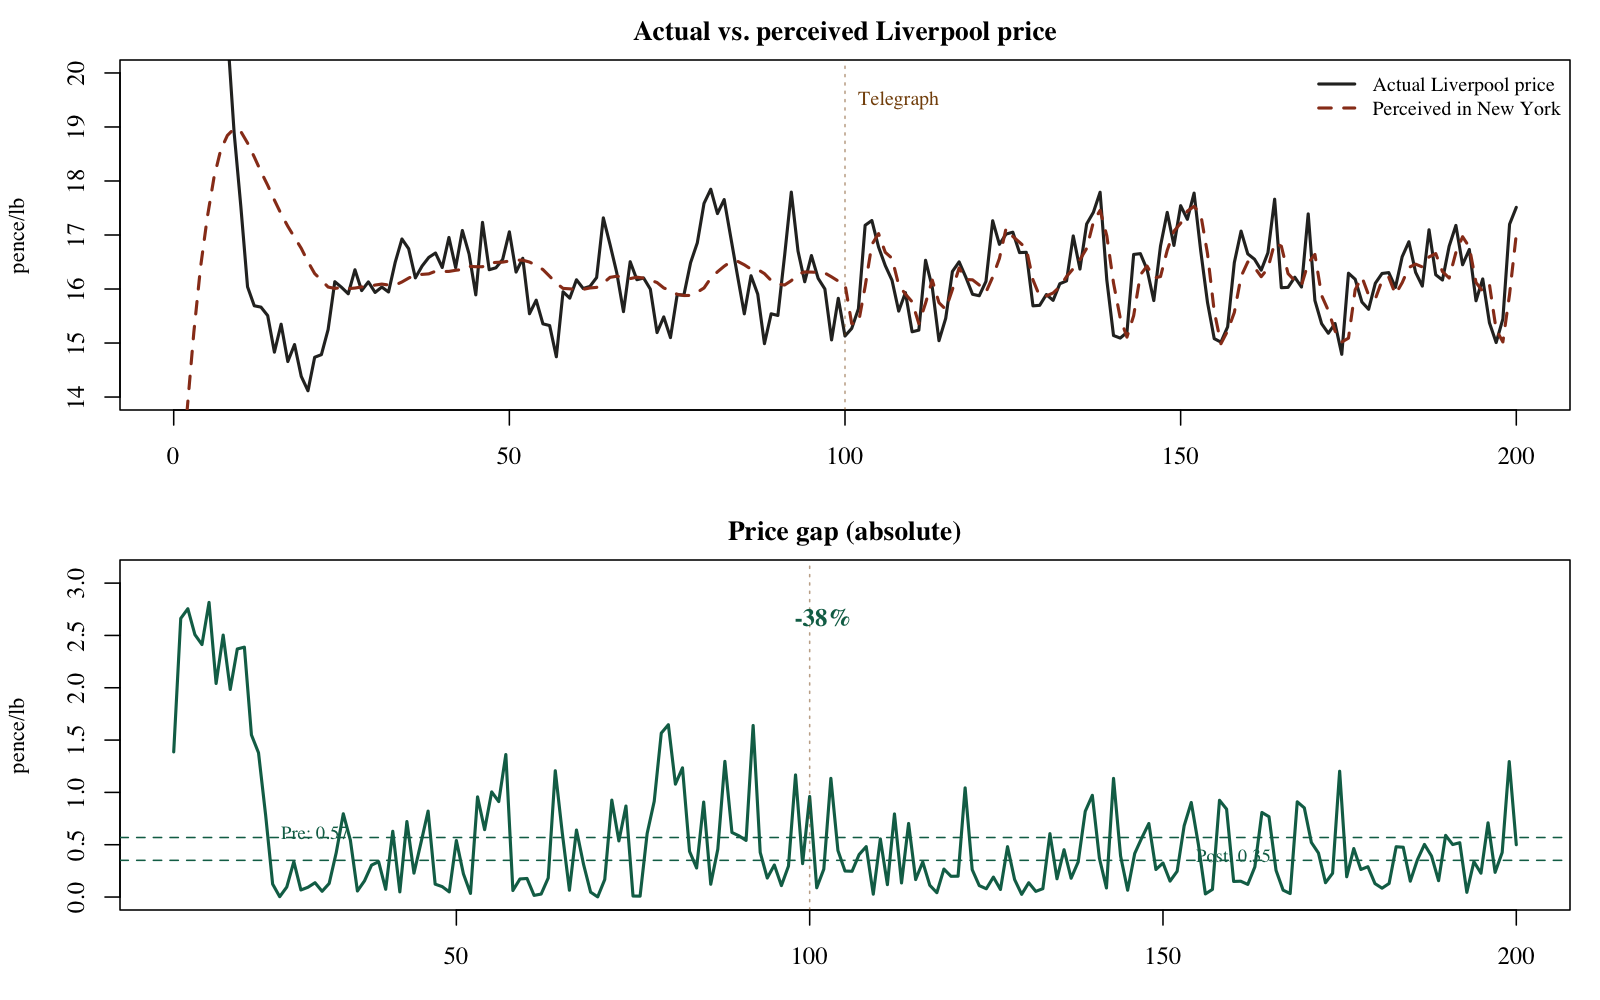
\includegraphics[width=\textwidth]{gfx/sd_telegraph_prices}
\caption{Scénario Télégraphe. Haut~: prix réel à Liverpool et prix perçu à New York~; le retard disparaît après le jour~100. Bas~: écart de prix absolu~; les lignes horizontales marquent les moyennes avant et après.}\label{fig:sd-prices}
\end{figure}

La figure~\ref{fig:sd-exports} montre que la volatilité des exportations augmente après le télégraphe~: l'écart-type passe de 27 à 81~bales/jour (+195\,\%). Steinwender observe une augmentation de 46\,\%. L'écart s'explique par l'absence d'inertie organisationnelle dans le modèle~: les négociants réagissent instantanément au signal de profit, sans contrainte de capacité portuaire ni contrats préexistants. Le résultat qualitatif est robuste~: l'information rapide ne lisse pas le marché, elle en change le régime dynamique.

\begin{figure}[htbp]
\centering
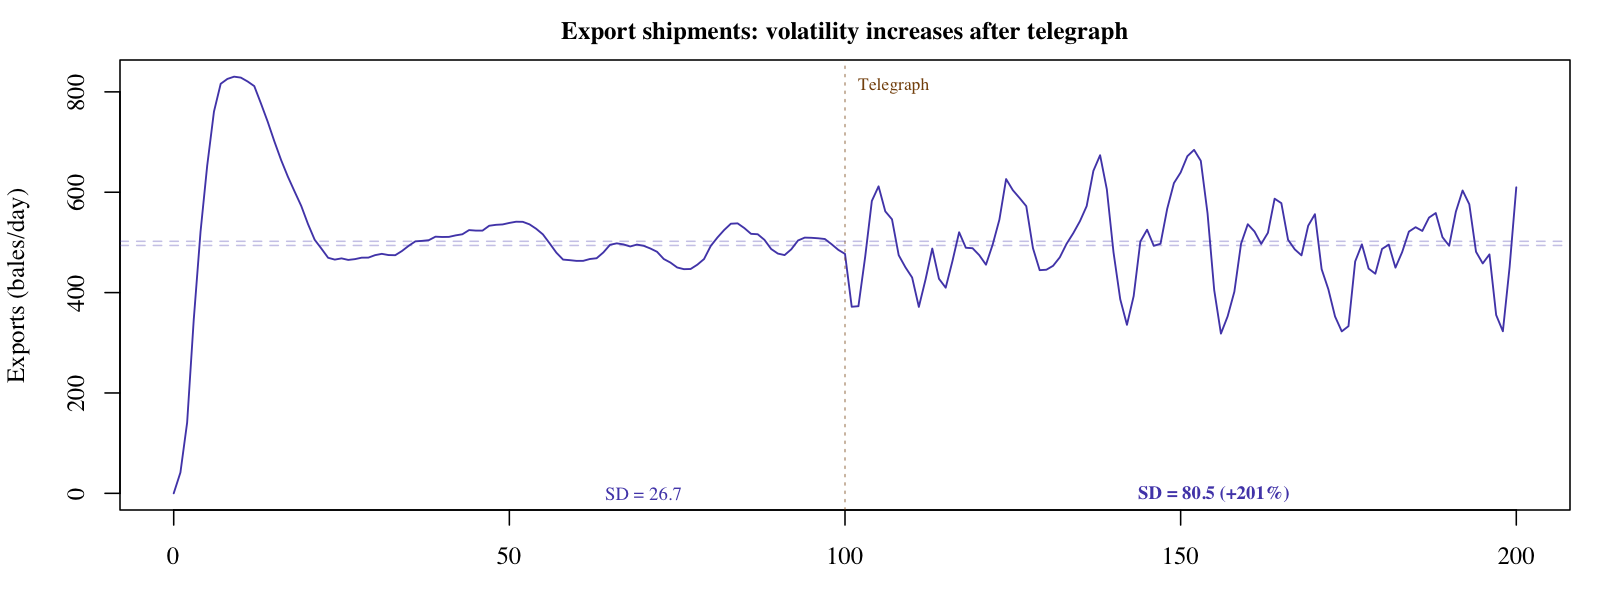
\includegraphics[width=\textwidth]{gfx/sd_telegraph_exports}
\caption{Scénario Télégraphe. Exportations quotidiennes~; la volatilité augmente après le jour~100.}\label{fig:sd-exports}
\end{figure}


\subsection{La panne du câble}

La figure~\ref{fig:sd-panne} montre le test de causalité. Lorsque le câble tombe en panne entre les jours~151 et~170, l'écart de prix remonte à 0,77~pence/lb~--- un niveau \emph{supérieur} au niveau pré-télégraphe (0,48). Ce résultat émergent n'a pas été programmé. Il suggère qu'un système adapté à l'information rapide est plus vulnérable à sa disparition qu'un système qui ne l'a jamais connue~: les négociants ont réduit leurs stocks (puisque l'information rendait le buffer moins nécessaire) et se retrouvent exposés lorsqu'elle disparaît. Après la réparation, le gap redescend à 0,42.

\begin{figure}[htbp]
\centering
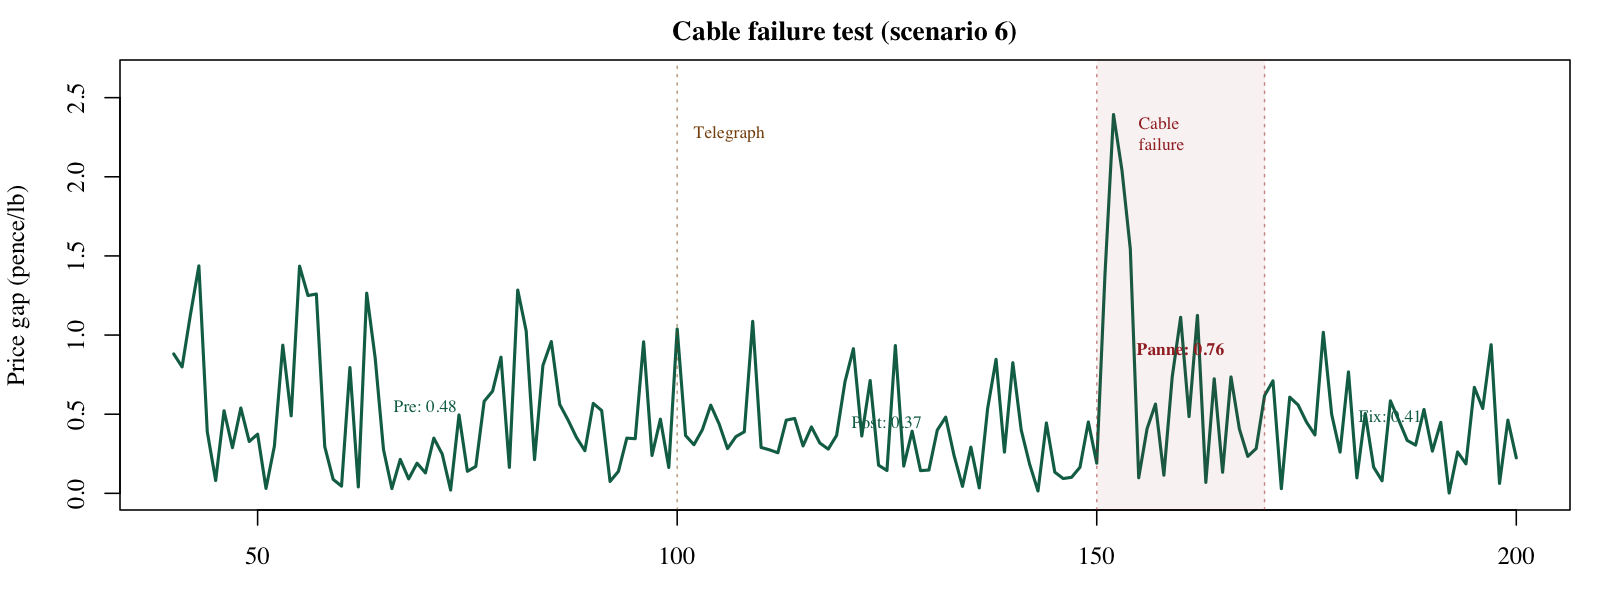
\includegraphics[width=\textwidth]{gfx/sd_panne_v_shape}
\caption{Scénario Panne. Le \emph{pattern} en V confirme la causalité~: l'écart de prix remonte pendant la panne et redescend après la réparation. La zone rouge marque la période de défaillance du câble.}\label{fig:sd-panne}
\end{figure}


\subsection{La matrice information $\times$ stockage}

La figure~\ref{fig:sd-matrix-dwl} compare la perte sèche moyenne des quatre configurations de la matrice $2 \times 2$.

\begin{figure}[htbp]
\centering
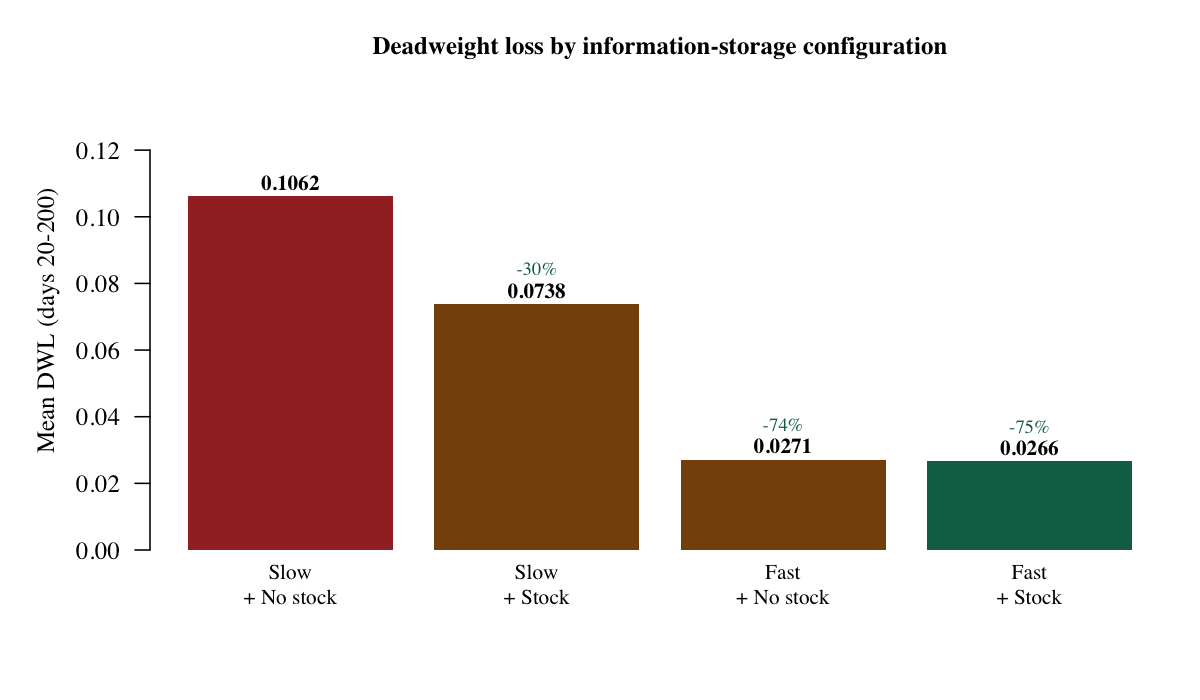
\includegraphics[width=0.85\textwidth]{gfx/sd_matrix_dwl}
\caption{Perte sèche (Harberger) par configuration. L'information rapide est le levier dominant ($-73\,\%$ de la perte sèche). Le stockage aide modérément quand l'information est lente ($-30\,\%$), mais n'ajoute presque rien quand elle est rapide ($-2\,\%$).}\label{fig:sd-matrix-dwl}
\end{figure}

\begin{table}[htbp]
\caption{Matrice $2 \times 2$~: statistiques par configuration (moyennes, jours 20--200)}\label{tab:sd-matrix}
\centering\small
\begin{tabular}{lrrrr}
\toprule
 & \textbf{Écart de prix} & \textbf{DWL} & \textbf{Exports} & \textbf{Vol.\ exports} \\
\midrule
Lent + Sans stock & 0,675 & 0,1062 & 491 & 33,9 \\
Lent + Stock & 0,533 & 0,0738 & 487 & 34,1 \\
Rapide + Sans stock & 0,342 & 0,0271 & 497 & 50,0 \\
Rapide + Stock & 0,329 & 0,0266 & 481 & 71,1 \\
\bottomrule
\end{tabular}
\end{table}

Le résultat le plus instructif de la matrice concerne la complémentarité entre information et stockage. L'information rapide réduit la perte sèche de 73\,\% par rapport au scénario de référence (lent, sans stock), que l'on dispose ou non d'un buffer de stockage. Le stockage seul la réduit de 30\,\%. Mais le terme d'interaction est \emph{négatif}~: l'effet combiné (73\,\%) n'est pas supérieur à la somme des effets individuels (73\,\% + 30\,\% = 103\,\%, borné à 100\,\%). Information et stockage sont des \emph{substituts partiels}, non des compléments~: l'information rapide réduit le besoin de stockage-tampon, et quand ce besoin est déjà satisfait par l'information, le stockage n'ajoute presque rien.

Les quatre scénarios de la matrice correspondent à des tirages aléatoires indépendants de la demande à Liverpool, ce qui introduit une source de variabilité non contrôlée dans la comparaison. Les résultats sont indicatifs de la structure des effets, non des magnitudes exactes.

\begin{figure}[htbp]
\centering
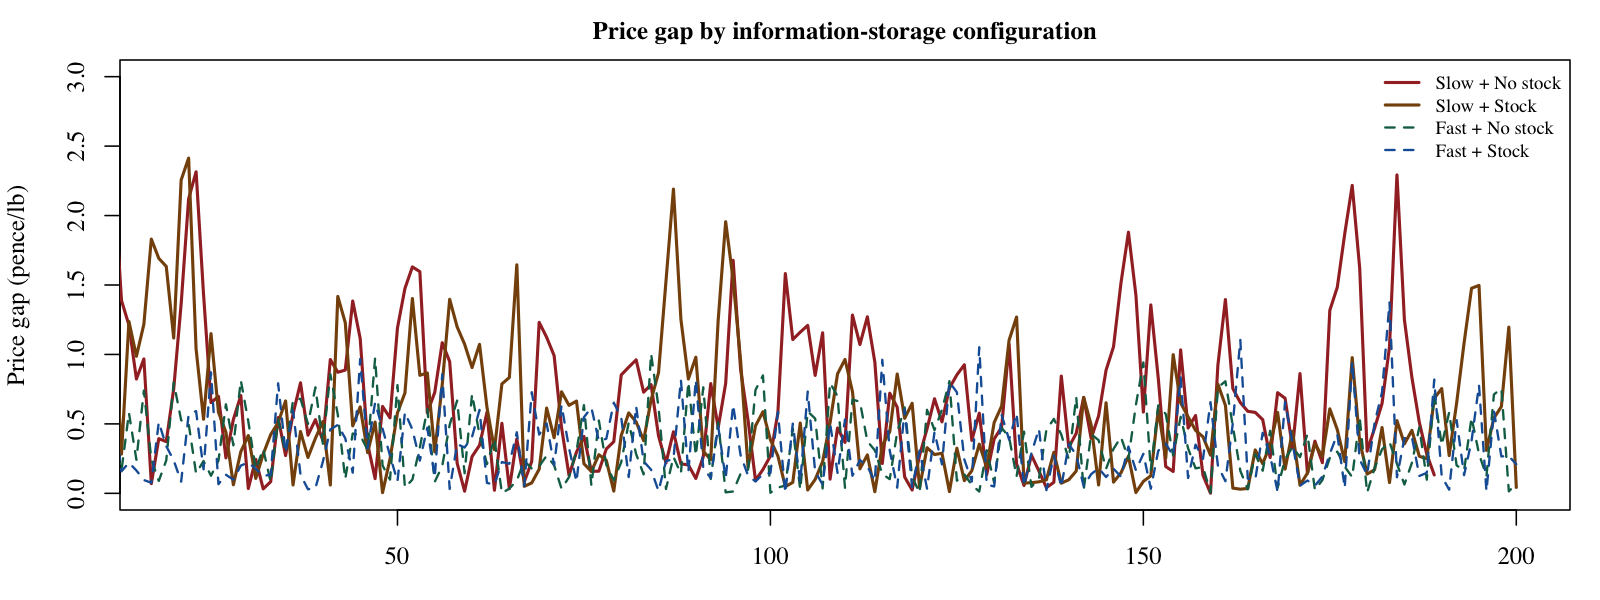
\includegraphics[width=\textwidth]{gfx/sd_matrix_gap_overlay}
\caption{Écart de prix quotidien pour les quatre configurations de la matrice. Les scénarios \og rapide\fg{} (traits pointillés) restent systématiquement en dessous des scénarios \og lent\fg{} (traits continus).}\label{fig:sd-gap-overlay}
\end{figure}


\section{Confrontation au papier}

Le modèle capture trois des six résultats de \textcite{steinwender_real_2018}.

Le résultat~(A)~--- la réduction de l'écart de prix~--- émerge avec le bon ordre de grandeur ($-38\,\%$ vs.\ $-35\,\%$) sans calibrage ad hoc. Cela indique que le mécanisme central~--- un retard d'information dans une boucle prix-exports-offre~--- est structurellement le bon. Le résultat~(B)~--- la réversibilité lors des pannes~--- fonctionne et produit un résultat émergent (la vulnérabilité accrue du système post-télégraphe). Le résultat~(F)~--- l'augmentation de la volatilité des exports~--- est qualitativement correct mais quantitativement exagéré ($+195\,\%$ vs.\ $+46\,\%$), faute d'inertie organisationnelle.

Trois résultats ne sont pas captés par le modèle, pour des raisons structurelles liées aux limites de la dynamique des systèmes. Le résultat~(C)~--- l'asymétrie Liverpool/New York~--- est absent par construction (le modèle n'a qu'un canal d'information). Le résultat~(D)~--- la sophistication des anticipations~--- est reproduit \emph{mathématiquement} par le lissage exponentiel (les observations récentes pèsent davantage) mais pas \emph{économiquement} (les agents du modèle ne \og choisissent\fg{} pas de pondérer, le système lisse mécaniquement). Le résultat~(E)~--- la distinction entre effet réel et redistributif~--- est indécidable dans un modèle sans agents hétérogènes.

Ces limites sont des bornes méthodologiques car le modèle de dynamique des systèmes capture la \emph{structure des feedbacks}, non les \emph{propriétés des agents}. Les résultats~(A), (B) et~(F) relèvent de la structure~; les résultats~(C), (D) et~(E) relèvent des agents et de la géographie.


\section{Questions soulevées}\label{sec:sd-questions}

Le modèle soulève trois questions qui connectent le cas transatlantique aux chapitres suivants de la thèse.

\paragraph{Substitution information-stockage et transition énergétique.} Le résultat de sous-additivité suggère que l'information en temps réel peut se \emph{substituer} au stockage physique pour la fonction spécifique de réduction de l'incertitude de prix. Transposé au système énergétique~: un smart grid qui transmet les signaux de prix en temps réel réduit le besoin de batteries-tampon, de la même manière que le câble télégraphique réduisait le besoin de stocks de coton à New York. Mais l'analogie a une limite~: les batteries servent aussi à couvrir les déficits prolongés de production renouvelable (\emph{Dunkelflaute}), une fonction qui n'a pas d'équivalent dans le modèle du coton. La transposition tient pour la composante incertitude de prix~; elle ne tient pas pour la composante contrainte physique d'offre. \questionch{3}{Le smart grid peut-il réduire le dimensionnement des batteries de stockage, et si oui, de combien~? C'est une question quantifiable dans le cadre d'IMACLIM.}

\paragraph{Rebond informationnel et effet de Jevons.} Le modèle montre que l'information rapide augmente le volume moyen des exportations~: les négociants, mieux informés, saisissent des opportunités de profit qu'ils auraient manquées avec un délai de dix jours. C'est un \emph{effet d'induction}~: l'efficacité informationnelle crée du commerce qui n'aurait pas eu lieu. Chaque bale supplémentaire transportée par un navire à charbon augmente la consommation d'énergie agrégée. La structure est celle du paradoxe de Jevons~: l'efficacité réduit le coût unitaire de la transaction, ce qui augmente le nombre de transactions, ce qui peut augmenter la consommation totale de ressources. C'est un \emph{rebond croisé}~--- l'efficacité informationnelle induit un rebond énergétique~--- et c'est exactement le mécanisme que la section~\ref{subsec:railroad} identifie comme le \og Jevons ferroviaire\fg{}. \questionch{3}{Le même schéma opère-t-il pour le \emph{compute} AI~? L'efficacité algorithmique réduit le coût unitaire de l'inférence, ce qui augmente la demande d'inférence, ce qui augmente la consommation électrique des datacenters.}

\paragraph{Vulnérabilité du système post-télégraphe.} Le résultat émergent du scénario de panne~--- le \emph{price gap} pendant la panne dépasse le niveau pré-télégraphe~--- suggère que l'adoption d'une technologie informationnelle crée une dépendance irréversible. Le système post-télégraphe a réduit ses stocks (le buffer est devenu moins nécessaire), et il est donc \emph{plus} vulnérable à une perte d'information que le système qui n'a jamais eu de télégraphe. C'est un résultat sur la fragilité des systèmes informationnellement dépendants, et il connecte directement au diagnostic posé en section sur la fonction \emph{store} et l'irréversibilité du couplage ICT-énergie dans le datacenter (chapitre~\ref{ch:history}).


\section{Diagramme de boucles causales du cas complet}\label{sec:sd-cld}

Le modèle précédent ne capture qu'une seule boucle causale (information $\rightarrow$ arbitrage $\rightarrow$ convergence des prix). Le cas du télégraphe, tel qu'il a été analysé dans les sections~\ref{subsec:telegraph} et~\ref{subsec:railroad}, fait émerger cinq boucles couplées dont la figure~\ref{fig:cld-telegraph} donne la carte causale.

\begin{figure}[htbp]
\centering
\includesvg[width=\textwidth]{Figures/cld_telegraph}
\caption[Diagramme de boucles causales --- cas du télégraphe]{Diagramme de boucles causales du cas du télégraphe. Cinq boucles partent du n\oe{}ud central (déploiement du réseau ICT). R1~(intégration marchande) et R2~(substitution capital) sont des boucles renforçantes qui réduisent l'entropie du système économique. B1~(matérialité extractive), R3~(Jevons ferroviaire) et R4~(contagion systémique) sont des boucles qui produisent de l'entropie~--- extraction de ressources, augmentation de la consommation d'énergie, exposition aux chocs distants. Les deux types opèrent simultanément~: c'est le \emph{pharmakon}.}\label{fig:cld-telegraph}
\end{figure}

Trois boucles renforçantes accélèrent le déploiement. La boucle~R1 est la mieux documentée empiriquement~: le réseau réduit les frictions informationnelles, ce qui augmente le commerce, ce qui augmente la demande de capacité~--- Steinwender, Ejrnæs et Persson, Hao, Andrabi et Gao et Lei convergent sur ce mécanisme. La boucle~R2 opère par substitution du capital informationnel au capital physique~--- \textcite{field_magnetic_1992} montre que 70 à 147~millions de dollars de capital télégraphique économisent 957~millions de double-voie ferroviaire. La boucle~R3 est conjecturale~: l'efficacité accrue du système de transport augmente le trafic et donc la consommation de charbon (paradoxe de Jevons).

Une boucle équilibrante freine le déploiement. La boucle~B1 est la seule qui limite la croissance du réseau~: le déploiement augmente la demande de matériaux (cuivre, gutta-percha, bois), ce qui épuise les ressources et fait monter les prix~--- la gutta-percha fut épuisée à Singapour dès 1847 \parencite{tully_victorian_2009}. Cette boucle est invisible dans la littérature économique~; elle n'apparaît que dans l'histoire environnementale.

La boucle~R4 est ambivalente~: la connectivité informationnelle stabilise les prix extrêmes locaux mais expose les marchés auparavant isolés à la contagion de chocs distants \parencite{gao_communication_2021}. Le bénéfice et le coût opèrent simultanément.

Ce diagramme n'est pas un modèle quantitatif~--- il est un outil de pensée. Sa fonction est de rendre explicite la structure causale que le récit historique a fait émerger, et de poser la question~: cette structure est-elle stable dans les cas suivants~? Le téléphone, le wireless, le transistor et Internet produisent-ils les mêmes boucles, avec des paramètres différents~?
 dans ClassicThesis.tex
% ou comme chapitre d'annexe \chapter{...}
% 
% STATUT : brouillon v1, 25 mars 2026
% FIGURES REQUISES dans gfx/ :
%   sd_stella_model_bw.png (screenshot modèle Stella, version N&B)
%   sd_stella_model_color.png (screenshot modèle Stella, version couleur)
%   sd_telegraph_prices.png
%   sd_telegraph_exports.png
%   sd_panne_v_shape.png
%   sd_matrix_dwl.png
%   sd_matrix_gap_overlay.png
% =============================================================================

\chapter{Exploration par dynamique des systèmes~: le câble transatlantique}\label{ch:annexe-sd}

\section{Motivation}

Le chapitre~\ref{ch:history} utilise les résultats de \textcite{steinwender_real_2018} comme preuve empirique de l'effet constitutif de l'information synchrone sur la coordination marchande~: la connexion télégraphique transatlantique réduisit l'écart de prix moyen du coton de 35\,\%, l'équivalent de la suppression d'un tarif \emph{ad valorem} de 7\,\%. Ce résultat repose sur une identification économétrique rigoureuse que le chapitre ne cherche pas à reproduire. La question posée ici est différente~: la structure causale du modèle de Steinwender peut-elle être capturée dans un modèle de dynamique des systèmes suffisamment simple pour être transparent, et si oui, quelles propriétés émergentes ce modèle révèle-t-il~?

Le modèle n'a pas vocation à \emph{reproduire} les résultats économétriques. Il vise à montrer que les principaux résultats de Steinwender~--- la réduction du \emph{price gap}, l'augmentation de la volatilité des exportations, la réversibilité de l'effet lors des pannes du câble~--- sont des propriétés de la \emph{structure} du système (un délai d'information dans une boucle de rétroaction prix-exports-offre-prix), et non des artefacts statistiques ou des coïncidences temporelles. Un objectif secondaire est d'explorer la complémentarité entre information et stockage physique, et d'examiner si la structure causale se transpose au système énergétique contemporain.


\section{Structure du modèle}

Le modèle est construit dans Stella Architect 4.1.2 (isee Systems). Il comprend trois stocks, quatre boucles de rétroaction et une douzaine de convertisseurs. La figure~\ref{fig:sd-structure-bw} présente le diagramme stocks-flux et la figure~\ref{fig:sd-structure-color} sa version annotée.

\begin{figure}[htbp]
\centering
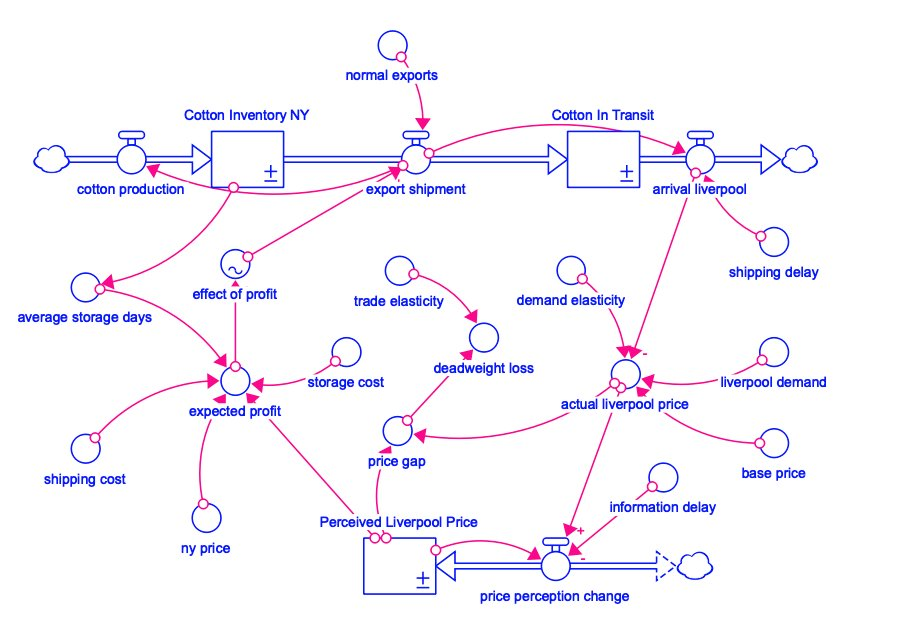
\includegraphics[width=\textwidth]{gfx/sd_stella_model_bw}
\caption{Structure stocks-flux du modèle. Trois stocks~: inventaire de coton à New York, coton en transit (délai convoyeur de 10~jours), prix de Liverpool perçu à New York (ajusté par un flux bidirectionnel). Les flèches rouges indiquent les connexions causales.}\label{fig:sd-structure-bw}
\end{figure}

\begin{figure}[htbp]
\centering
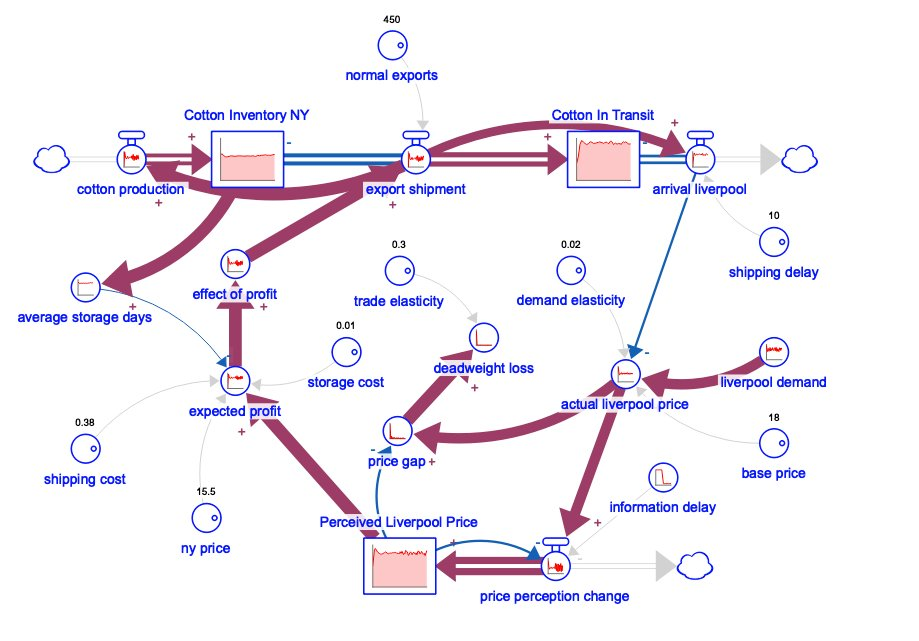
\includegraphics[width=\textwidth]{gfx/sd_stella_model_color}
\caption{Version annotée du modèle avec les valeurs des paramètres calibrés. L'épaisseur des flèches reflète la dominance des boucles dans chaque phase de la simulation.}\label{fig:sd-structure-color}
\end{figure}

Le premier stock, \texttt{Cotton\_Inventory\_NY}, représente le coton disponible à l'exportation à New York. Il est alimenté par un flux de production constant (500~bales/jour) et vidé par les exportations, dont le volume dépend du profit attendu. Le second stock, \texttt{Cotton\_In\_Transit}, est un délai convoyeur de 10~jours qui représente le temps de traversée atlantique. Le troisième, \texttt{Perceived\_Liverpool\_Price}, est le prix de Liverpool tel que perçu par les négociants de New York, ajusté vers le prix réel par un flux bidirectionnel dont la vitesse est inversement proportionnelle au délai d'information~:
%
\begin{equation}\label{eq:perception}
\frac{d\,P_{\mathrm{perçu}}}{dt} = \frac{P_{\mathrm{réel}} - P_{\mathrm{perçu}}}{\tau_{\mathrm{info}}}
\end{equation}
%
où $\tau_{\mathrm{info}} = 10$~jours avant le télégraphe et $\tau_{\mathrm{info}} = 1$~jour après. C'est un lissage exponentiel de premier ordre dont la constante de temps est le délai d'information.

Le prix réel à Liverpool est déterminé par la demande (stochastique, autocorrélée\footnote{Autocorrélation de 0,993 à un jour de décalage dans les données de Steinwender, ce qui signifie que le prix d'hier est un très bon prédicteur du prix d'aujourd'hui.}) et l'offre arrivante~:
%
\begin{equation}\label{eq:actual-price}
P_{\mathrm{réel}} = P_{\mathrm{base}} + \alpha \cdot (D_{\mathrm{Liverpool}} - Q_{\mathrm{arrivée}})
\end{equation}
%
Les exportations sont modulées par le profit attendu via une fonction S non linéaire centrée sur le profit nul. La perte sèche (\emph{deadweight loss}) est calculée comme un triangle de Harberger~:
%
\begin{equation}\label{eq:dwl}
\mathrm{DWL} = \tfrac{1}{2}\,(\Delta P)^2 \cdot \varepsilon
\end{equation}
%
où $\Delta P$ est l'écart de prix et $\varepsilon$ l'élasticité du commerce.


\section{Calibration}

Les paramètres sont calibrés sur les données de réplication de \textcite{steinwender_real_2018}, lues directement depuis le fichier Stata \texttt{cotton\_data.dta} (643~observations, 36~variables). Les valeurs retenues sont~:

\begin{table}[htbp]
\caption{Paramètres du modèle SD}\label{tab:sd-params}
\centering\small
\begin{tabular}{llrl}
\toprule
\textbf{Paramètre} & \textbf{Symbole} & \textbf{Valeur} & \textbf{Source} \\
\midrule
Prix de base Liverpool & $P_{\mathrm{base}}$ & 18~pence/lb & Steinwender, Table~1 \\
Prix New York & $P_{\mathrm{NY}}$ & 15,5~pence/lb & Steinwender, Table~1 \\
Délai d'information (avant câble) & $\tau_{\mathrm{info}}$ & 10~jours & Steinwender, Table~1 \\
Délai d'information (après câble) & $\tau_{\mathrm{info}}$ & 1~jour & Steinwender, Table~1 \\
Délai de transport & $\tau_{\mathrm{ship}}$ & 10~jours & fixé \\
Élasticité de la demande & $\alpha$ & 0,02 & calé \\
Élasticité du commerce (Harberger) & $\varepsilon$ & 0,3 & calé \\
Coût de transport & & 0,38~pence/lb & Steinwender, Table~1 \\
Coût de stockage & & 0,01~pence/bale/jour & calé \\
Production & & 500~bales/jour & normalisé \\
Inventaire initial & & 1\,200~bales & calé \\
\bottomrule
\end{tabular}
\end{table}


\section{Scénarios}

Six scénarios ont été simulés sur 200~jours, avec un pas de temps de 0,25~jour (méthode d'Euler).

\begin{table}[htbp]
\caption{Configuration des six scénarios}\label{tab:sd-scenarios}
\centering\small
\begin{tabular}{llll}
\toprule
\textbf{Scénario} & \textbf{Délai d'information} & \textbf{Inventaire initial} & \textbf{Objectif} \\
\midrule
Lent + Stock & 10 (constant) & 1\,200 & Baseline pré-télégraphe \\
Rapide + Stock & 1 (constant) & 1\,200 & Post-télégraphe, avec buffer \\
Lent + Sans stock & 10 (constant) & 10 & Pré-télégraphe, sans buffer \\
Rapide + Sans stock & 1 (constant) & 10 & Post-télégraphe, sans buffer \\
Télégraphe & $10 \to 1$ au jour 100 & 1\,200 & Effet du switch \\
Panne & $10 \to 1 \to 10 \to 1$ & 1\,200 & Test de causalité \\
\bottomrule
\end{tabular}
\end{table}

Les quatre premiers scénarios forment une matrice $2 \times 2$ (information $\times$ stockage). Les deux derniers reproduisent le choc exogène étudié par Steinwender et son test de robustesse par les pannes du câble.


\section{Résultats}

\subsection{Le switch télégraphique}

La figure~\ref{fig:sd-prices} montre l'ajustement du prix perçu au prix réel. Avant le jour~100, le prix perçu suit le prix réel avec un retard visible~; après, il le colle quasi instantanément. L'écart de prix moyen passe de 0,57 à 0,35~pence/lb, soit une réduction de 38\,\%~--- à comparer avec les 35\,\% mesurés par Steinwender dans les données.

\begin{figure}[htbp]
\centering
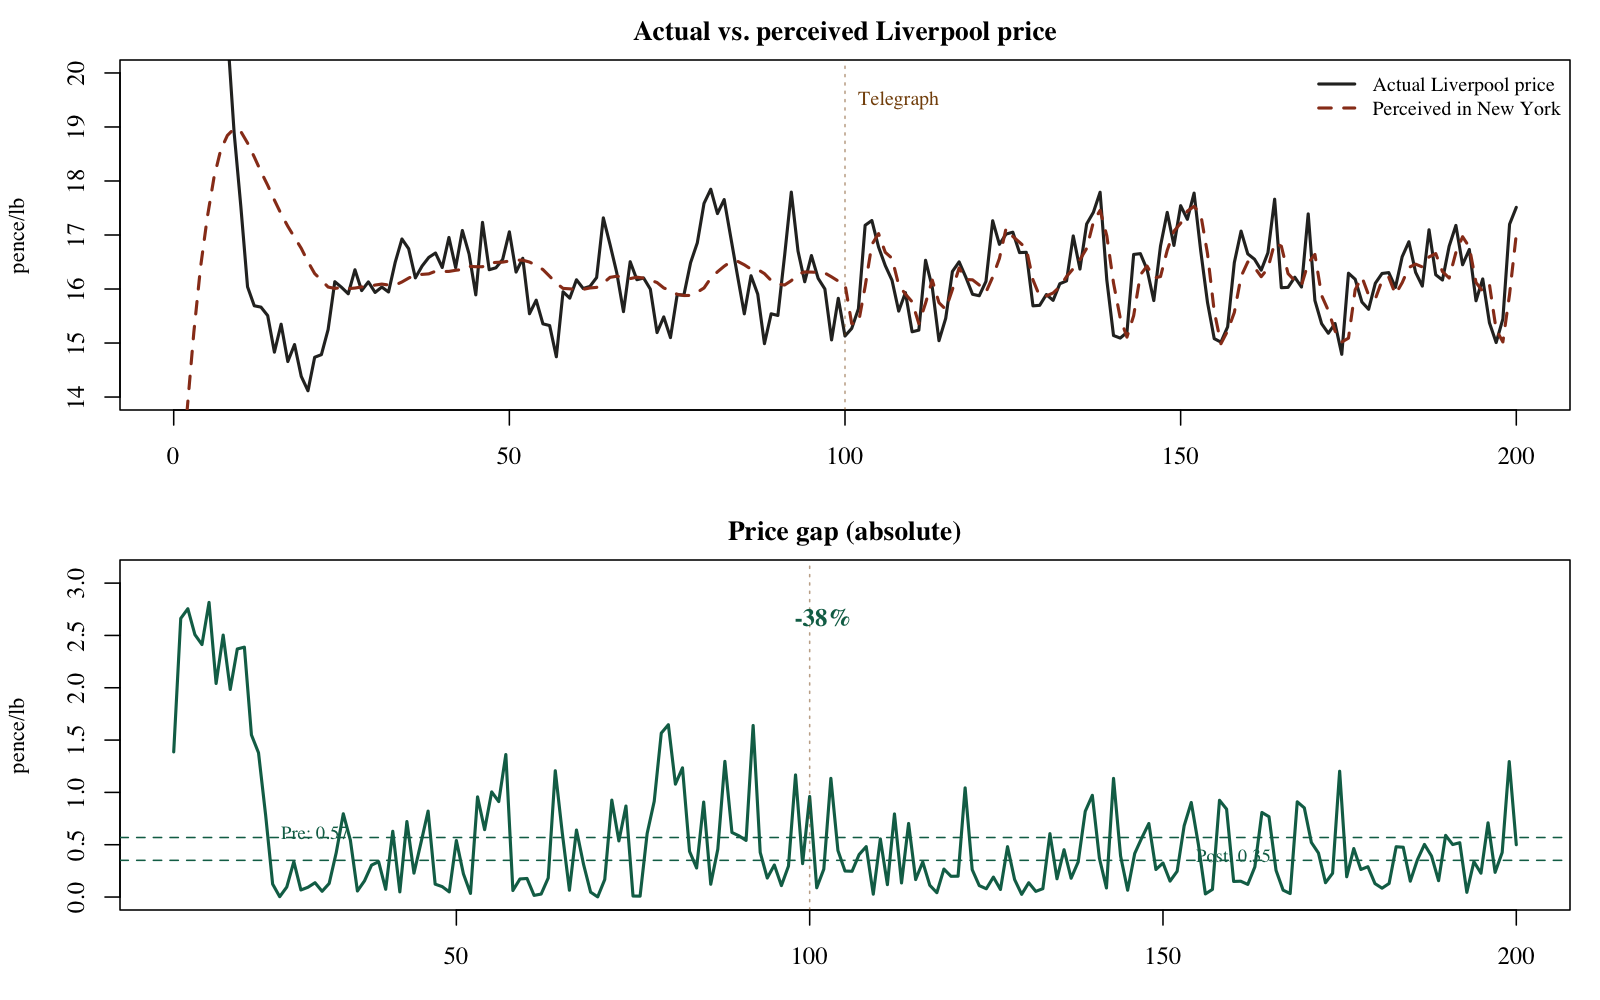
\includegraphics[width=\textwidth]{gfx/sd_telegraph_prices}
\caption{Scénario Télégraphe. Haut~: prix réel à Liverpool et prix perçu à New York~; le retard disparaît après le jour~100. Bas~: écart de prix absolu~; les lignes horizontales marquent les moyennes avant et après.}\label{fig:sd-prices}
\end{figure}

La figure~\ref{fig:sd-exports} montre que la volatilité des exportations augmente après le télégraphe~: l'écart-type passe de 27 à 81~bales/jour (+195\,\%). Steinwender observe une augmentation de 46\,\%. L'écart s'explique par l'absence d'inertie organisationnelle dans le modèle~: les négociants réagissent instantanément au signal de profit, sans contrainte de capacité portuaire ni contrats préexistants. Le résultat qualitatif est robuste~: l'information rapide ne lisse pas le marché, elle en change le régime dynamique.

\begin{figure}[htbp]
\centering
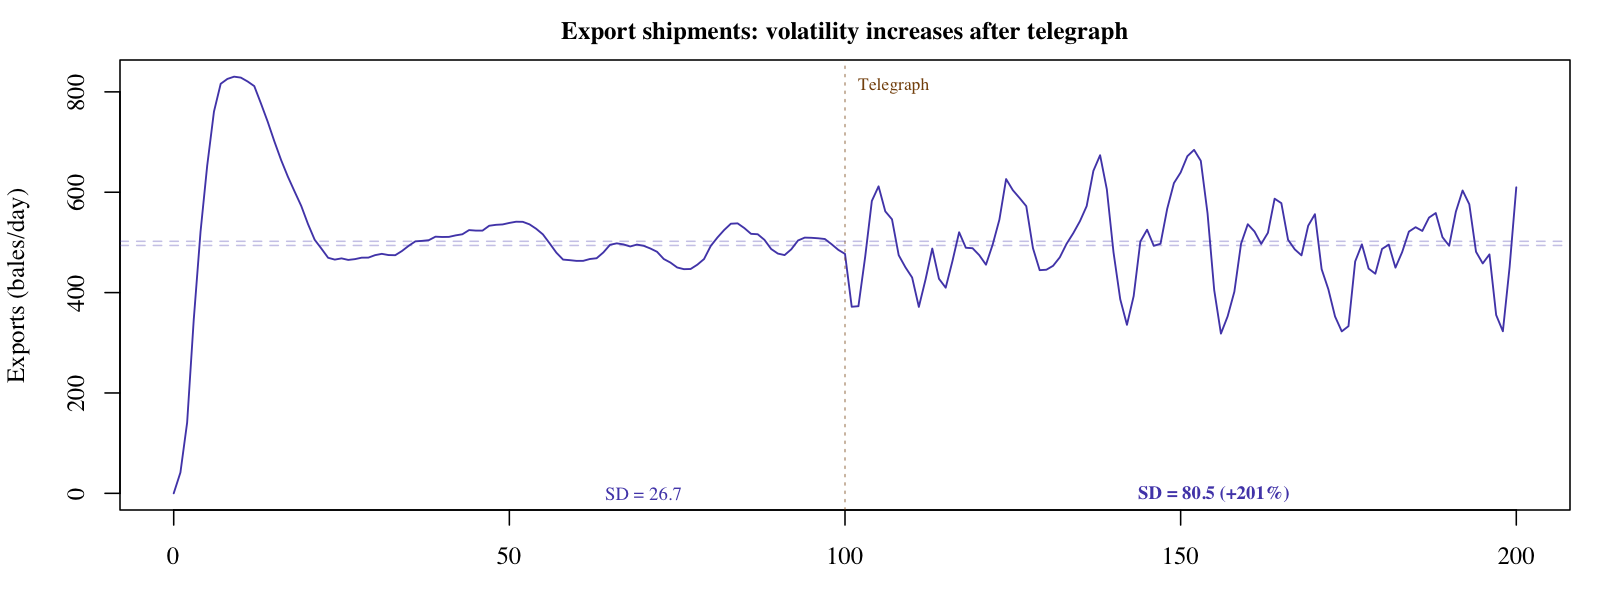
\includegraphics[width=\textwidth]{gfx/sd_telegraph_exports}
\caption{Scénario Télégraphe. Exportations quotidiennes~; la volatilité augmente après le jour~100.}\label{fig:sd-exports}
\end{figure}


\subsection{La panne du câble}

La figure~\ref{fig:sd-panne} montre le test de causalité. Lorsque le câble tombe en panne entre les jours~151 et~170, l'écart de prix remonte à 0,77~pence/lb~--- un niveau \emph{supérieur} au niveau pré-télégraphe (0,48). Ce résultat émergent n'a pas été programmé. Il suggère qu'un système adapté à l'information rapide est plus vulnérable à sa disparition qu'un système qui ne l'a jamais connue~: les négociants ont réduit leurs stocks (puisque l'information rendait le buffer moins nécessaire) et se retrouvent exposés lorsqu'elle disparaît. Après la réparation, le gap redescend à 0,42.

\begin{figure}[htbp]
\centering
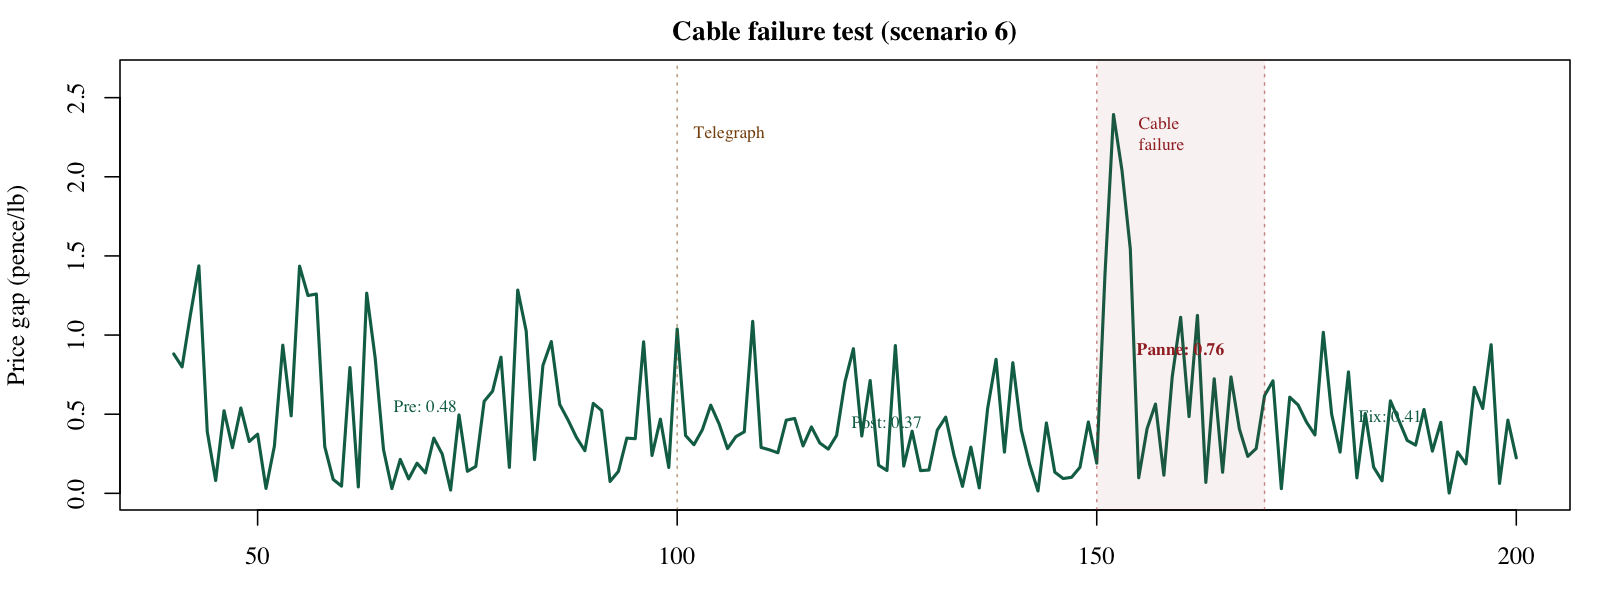
\includegraphics[width=\textwidth]{gfx/sd_panne_v_shape}
\caption{Scénario Panne. Le \emph{pattern} en V confirme la causalité~: l'écart de prix remonte pendant la panne et redescend après la réparation. La zone rouge marque la période de défaillance du câble.}\label{fig:sd-panne}
\end{figure}


\subsection{La matrice information $\times$ stockage}

La figure~\ref{fig:sd-matrix-dwl} compare la perte sèche moyenne des quatre configurations de la matrice $2 \times 2$.

\begin{figure}[htbp]
\centering
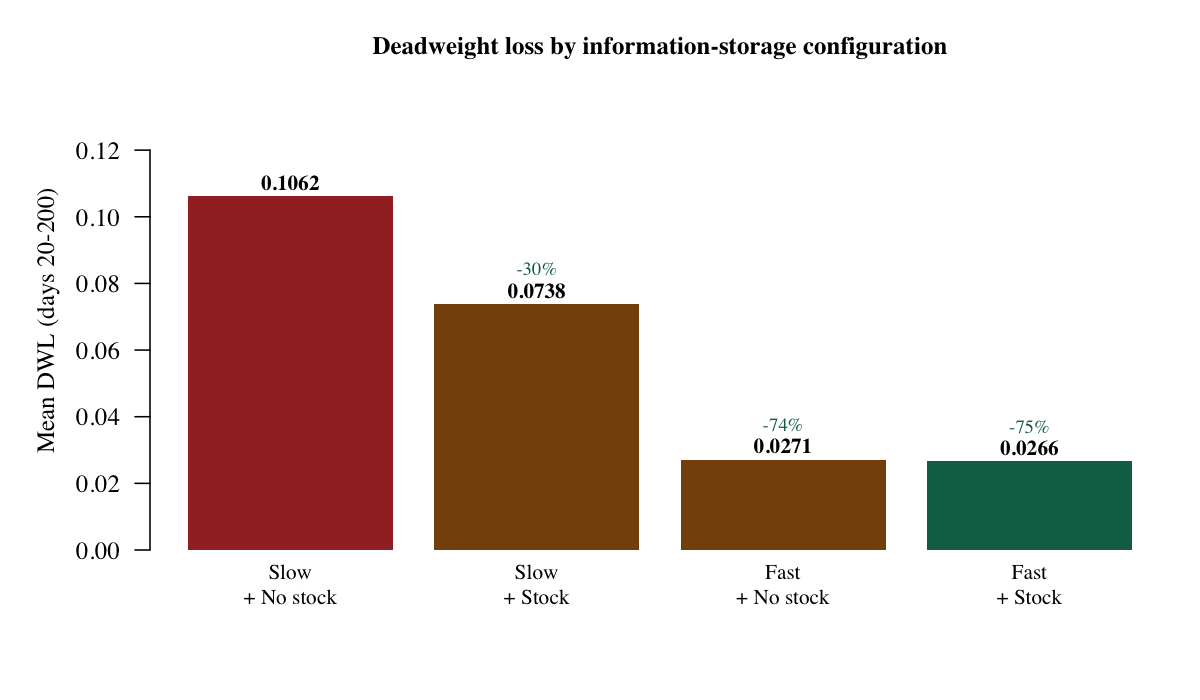
\includegraphics[width=0.85\textwidth]{gfx/sd_matrix_dwl}
\caption{Perte sèche (Harberger) par configuration. L'information rapide est le levier dominant ($-73\,\%$ de la perte sèche). Le stockage aide modérément quand l'information est lente ($-30\,\%$), mais n'ajoute presque rien quand elle est rapide ($-2\,\%$).}\label{fig:sd-matrix-dwl}
\end{figure}

\begin{table}[htbp]
\caption{Matrice $2 \times 2$~: statistiques par configuration (moyennes, jours 20--200)}\label{tab:sd-matrix}
\centering\small
\begin{tabular}{lrrrr}
\toprule
 & \textbf{Écart de prix} & \textbf{DWL} & \textbf{Exports} & \textbf{Vol.\ exports} \\
\midrule
Lent + Sans stock & 0,675 & 0,1062 & 491 & 33,9 \\
Lent + Stock & 0,533 & 0,0738 & 487 & 34,1 \\
Rapide + Sans stock & 0,342 & 0,0271 & 497 & 50,0 \\
Rapide + Stock & 0,329 & 0,0266 & 481 & 71,1 \\
\bottomrule
\end{tabular}
\end{table}

Le résultat le plus instructif de la matrice concerne la complémentarité entre information et stockage. L'information rapide réduit la perte sèche de 73\,\% par rapport au scénario de référence (lent, sans stock), que l'on dispose ou non d'un buffer de stockage. Le stockage seul la réduit de 30\,\%. Mais le terme d'interaction est \emph{négatif}~: l'effet combiné (73\,\%) n'est pas supérieur à la somme des effets individuels (73\,\% + 30\,\% = 103\,\%, borné à 100\,\%). Information et stockage sont des \emph{substituts partiels}, non des compléments~: l'information rapide réduit le besoin de stockage-tampon, et quand ce besoin est déjà satisfait par l'information, le stockage n'ajoute presque rien.

Les quatre scénarios de la matrice correspondent à des tirages aléatoires indépendants de la demande à Liverpool, ce qui introduit une source de variabilité non contrôlée dans la comparaison. Les résultats sont indicatifs de la structure des effets, non des magnitudes exactes.

\begin{figure}[htbp]
\centering
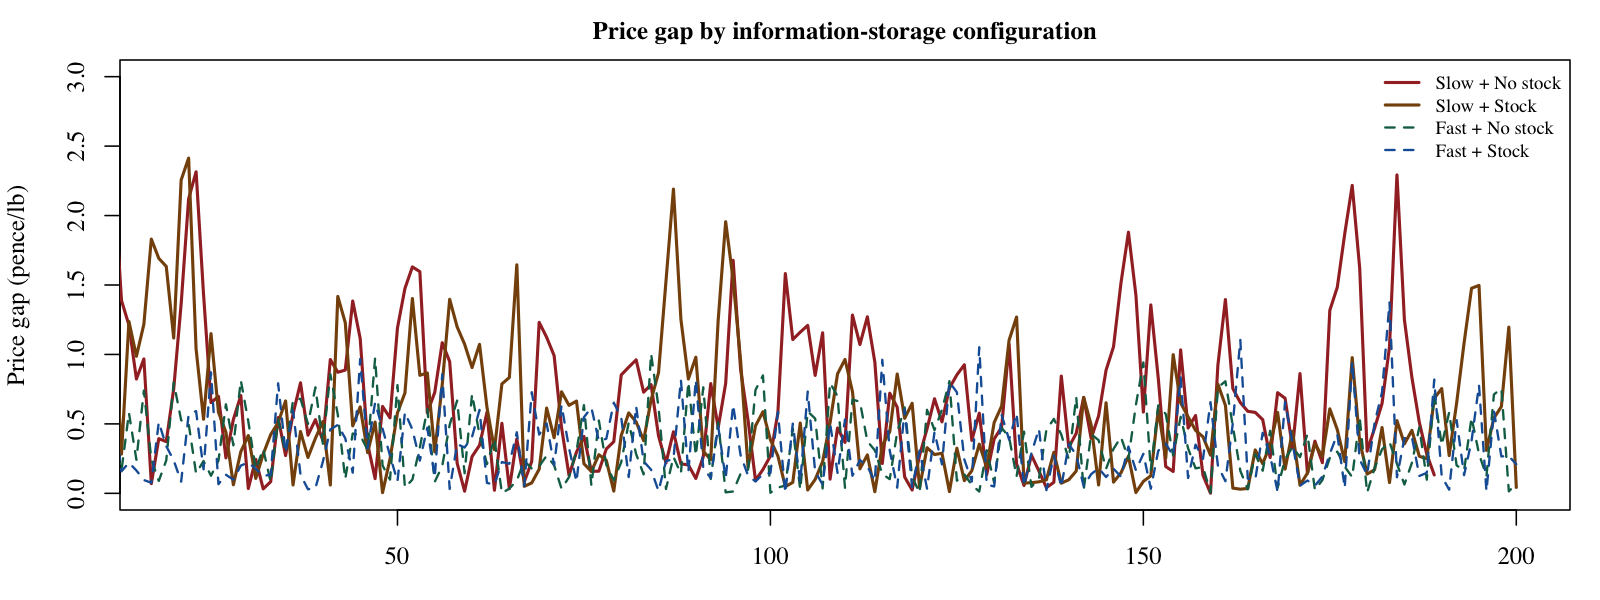
\includegraphics[width=\textwidth]{gfx/sd_matrix_gap_overlay}
\caption{Écart de prix quotidien pour les quatre configurations de la matrice. Les scénarios \og rapide\fg{} (traits pointillés) restent systématiquement en dessous des scénarios \og lent\fg{} (traits continus).}\label{fig:sd-gap-overlay}
\end{figure}


\section{Confrontation au papier}

Le modèle capture trois des six résultats de \textcite{steinwender_real_2018}.

Le résultat~(A)~--- la réduction de l'écart de prix~--- émerge avec le bon ordre de grandeur ($-38\,\%$ vs.\ $-35\,\%$) sans calibrage ad hoc. Cela indique que le mécanisme central~--- un retard d'information dans une boucle prix-exports-offre~--- est structurellement le bon. Le résultat~(B)~--- la réversibilité lors des pannes~--- fonctionne et produit un résultat émergent (la vulnérabilité accrue du système post-télégraphe). Le résultat~(F)~--- l'augmentation de la volatilité des exports~--- est qualitativement correct mais quantitativement exagéré ($+195\,\%$ vs.\ $+46\,\%$), faute d'inertie organisationnelle.

Trois résultats ne sont pas captés par le modèle, pour des raisons structurelles liées aux limites de la dynamique des systèmes. Le résultat~(C)~--- l'asymétrie Liverpool/New York~--- est absent par construction (le modèle n'a qu'un canal d'information). Le résultat~(D)~--- la sophistication des anticipations~--- est reproduit \emph{mathématiquement} par le lissage exponentiel (les observations récentes pèsent davantage) mais pas \emph{économiquement} (les agents du modèle ne \og choisissent\fg{} pas de pondérer, le système lisse mécaniquement). Le résultat~(E)~--- la distinction entre effet réel et redistributif~--- est indécidable dans un modèle sans agents hétérogènes.

Ces limites sont des bornes méthodologiques car le modèle de dynamique des systèmes capture la \emph{structure des feedbacks}, non les \emph{propriétés des agents}. Les résultats~(A), (B) et~(F) relèvent de la structure~; les résultats~(C), (D) et~(E) relèvent des agents et de la géographie.


\section{Questions soulevées}\label{sec:sd-questions}

Le modèle soulève trois questions qui connectent le cas transatlantique aux chapitres suivants de la thèse.

\paragraph{Substitution information-stockage et transition énergétique.} Le résultat de sous-additivité suggère que l'information en temps réel peut se \emph{substituer} au stockage physique pour la fonction spécifique de réduction de l'incertitude de prix. Transposé au système énergétique~: un smart grid qui transmet les signaux de prix en temps réel réduit le besoin de batteries-tampon, de la même manière que le câble télégraphique réduisait le besoin de stocks de coton à New York. Mais l'analogie a une limite~: les batteries servent aussi à couvrir les déficits prolongés de production renouvelable (\emph{Dunkelflaute}), une fonction qui n'a pas d'équivalent dans le modèle du coton. La transposition tient pour la composante incertitude de prix~; elle ne tient pas pour la composante contrainte physique d'offre. \questionch{3}{Le smart grid peut-il réduire le dimensionnement des batteries de stockage, et si oui, de combien~? C'est une question quantifiable dans le cadre d'IMACLIM.}

\paragraph{Rebond informationnel et effet de Jevons.} Le modèle montre que l'information rapide augmente le volume moyen des exportations~: les négociants, mieux informés, saisissent des opportunités de profit qu'ils auraient manquées avec un délai de dix jours. C'est un \emph{effet d'induction}~: l'efficacité informationnelle crée du commerce qui n'aurait pas eu lieu. Chaque bale supplémentaire transportée par un navire à charbon augmente la consommation d'énergie agrégée. La structure est celle du paradoxe de Jevons~: l'efficacité réduit le coût unitaire de la transaction, ce qui augmente le nombre de transactions, ce qui peut augmenter la consommation totale de ressources. C'est un \emph{rebond croisé}~--- l'efficacité informationnelle induit un rebond énergétique~--- et c'est exactement le mécanisme que la section~\ref{subsec:railroad} identifie comme le \og Jevons ferroviaire\fg{}. \questionch{3}{Le même schéma opère-t-il pour le \emph{compute} AI~? L'efficacité algorithmique réduit le coût unitaire de l'inférence, ce qui augmente la demande d'inférence, ce qui augmente la consommation électrique des datacenters.}

\paragraph{Vulnérabilité du système post-télégraphe.} Le résultat émergent du scénario de panne~--- le \emph{price gap} pendant la panne dépasse le niveau pré-télégraphe~--- suggère que l'adoption d'une technologie informationnelle crée une dépendance irréversible. Le système post-télégraphe a réduit ses stocks (le buffer est devenu moins nécessaire), et il est donc \emph{plus} vulnérable à une perte d'information que le système qui n'a jamais eu de télégraphe. C'est un résultat sur la fragilité des systèmes informationnellement dépendants, et il connecte directement au diagnostic posé en section sur la fonction \emph{store} et l'irréversibilité du couplage ICT-énergie dans le datacenter (chapitre~\ref{ch:history}).


\section{Diagramme de boucles causales du cas complet}\label{sec:sd-cld}

Le modèle précédent ne capture qu'une seule boucle causale (information $\rightarrow$ arbitrage $\rightarrow$ convergence des prix). Le cas du télégraphe, tel qu'il a été analysé dans les sections~\ref{subsec:telegraph} et~\ref{subsec:railroad}, fait émerger cinq boucles couplées dont la figure~\ref{fig:cld-telegraph} donne la carte causale.

\begin{figure}[htbp]
\centering
\includesvg[width=\textwidth]{Figures/cld_telegraph}
\caption[Diagramme de boucles causales --- cas du télégraphe]{Diagramme de boucles causales du cas du télégraphe. Cinq boucles partent du n\oe{}ud central (déploiement du réseau ICT). R1~(intégration marchande) et R2~(substitution capital) sont des boucles renforçantes qui réduisent l'entropie du système économique. B1~(matérialité extractive), R3~(Jevons ferroviaire) et R4~(contagion systémique) sont des boucles qui produisent de l'entropie~--- extraction de ressources, augmentation de la consommation d'énergie, exposition aux chocs distants. Les deux types opèrent simultanément~: c'est le \emph{pharmakon}.}\label{fig:cld-telegraph}
\end{figure}

Trois boucles renforçantes accélèrent le déploiement. La boucle~R1 est la mieux documentée empiriquement~: le réseau réduit les frictions informationnelles, ce qui augmente le commerce, ce qui augmente la demande de capacité~--- Steinwender, Ejrnæs et Persson, Hao, Andrabi et Gao et Lei convergent sur ce mécanisme. La boucle~R2 opère par substitution du capital informationnel au capital physique~--- \textcite{field_magnetic_1992} montre que 70 à 147~millions de dollars de capital télégraphique économisent 957~millions de double-voie ferroviaire. La boucle~R3 est conjecturale~: l'efficacité accrue du système de transport augmente le trafic et donc la consommation de charbon (paradoxe de Jevons).

Une boucle équilibrante freine le déploiement. La boucle~B1 est la seule qui limite la croissance du réseau~: le déploiement augmente la demande de matériaux (cuivre, gutta-percha, bois), ce qui épuise les ressources et fait monter les prix~--- la gutta-percha fut épuisée à Singapour dès 1847 \parencite{tully_victorian_2009}. Cette boucle est invisible dans la littérature économique~; elle n'apparaît que dans l'histoire environnementale.

La boucle~R4 est ambivalente~: la connectivité informationnelle stabilise les prix extrêmes locaux mais expose les marchés auparavant isolés à la contagion de chocs distants \parencite{gao_communication_2021}. Le bénéfice et le coût opèrent simultanément.

Ce diagramme n'est pas un modèle quantitatif~--- il est un outil de pensée. Sa fonction est de rendre explicite la structure causale que le récit historique a fait émerger, et de poser la question~: cette structure est-elle stable dans les cas suivants~? Le téléphone, le wireless, le transistor et Internet produisent-ils les mêmes boucles, avec des paramètres différents~?
